\chapter{Results and Discussion}
For the development phase of the project 1 Dataset has been used for training namely: 
\begin{itemize}
    \item \href{https://www.kaggle.com/datasets/sartajbhuvaji/brain-tumor-classification-mri}{Brain Tumor Classification (MRI)}
\end{itemize}
The dataset is divided into four labels: Glioma, Meningioma, No Tumour and Pituitary tumour. This data is then shuffled using shuffle command of keras. All this data was then passed onto a final dataset, which was then separated into 3 segments: Train , Test and Validation in ratio of 80:10:10. Once the data has been split, a pre-trained model is imported and on top of that pre-trained layers, we add new training layers for the task being performed. This concept is known as transfer learning. Then these train images are passed on to the model. The model has been trained for 19 versions, where each version differs in the pre-trained model being imported. These results associated with each version can be understood in the section \ref{section:results}. Based on the results from each verion the highest accuracy achieved is 97\% .

\section{Dataset Information}
Table \ref{tab:Dataset_info_chap5} displays the number of imgaes in the dataset.
\begin{table}[h!]
                \caption{Contents of Brain MRI Images for Brain Tumor Detection Dataset}
                \label{tab:Dataset_info_chap5}
\begin{tabular}{c|c|c|}
\cline{2-3}
\multicolumn{1}{l|}{}                                                                                                        & \cellcolor[HTML]{CBCEFB}\textbf{Data Label} & \cellcolor[HTML]{CBCEFB}\textbf{No. Of Images} \\ \hline
\multicolumn{1}{|c|}{\cellcolor[HTML]{CBCEFB}}                                                                               & Glioma                                      & 100                                            \\ \cline{2-3} 
\multicolumn{1}{|c|}{\cellcolor[HTML]{CBCEFB}}                                                                               & Meningioma                                  & 115                                            \\ \cline{2-3} 
\multicolumn{1}{|c|}{\cellcolor[HTML]{CBCEFB}}                                                                               & No Tumour                                   & 105                                            \\ \cline{2-3} 
\multicolumn{1}{|c|}{\multirow{-4}{*}{\cellcolor[HTML]{CBCEFB}\textbf{\begin{tabular}[c]{@{}c@{}}Test\\ Set\end{tabular}}}}  & Pituitary                                   & 74                                             \\ \hline
\multicolumn{1}{|c|}{\cellcolor[HTML]{CBCEFB}}                                                                               & Glioma                                      & 826                                            \\ \cline{2-3} 
\multicolumn{1}{|c|}{\cellcolor[HTML]{CBCEFB}}                                                                               & Meningioma                                  & 822                                            \\ \cline{2-3} 
\multicolumn{1}{|c|}{\cellcolor[HTML]{CBCEFB}}                                                                               & No Tumour                                   & 395                                            \\ \cline{2-3} 
\multicolumn{1}{|c|}{\multirow{-4}{*}{\cellcolor[HTML]{CBCEFB}\textbf{\begin{tabular}[c]{@{}c@{}}Train\\ Set\end{tabular}}}} & Pituitary                                   & 827                                            \\ \hline
\end{tabular}%
\end{table}

\section{Sample Data from Dataset}
Figure (\ref{fig:data_sample1}) plots some sample images from the dataset. These images are generated using a random function and the matplotlib library. One image from each label (Glioma, No Tumour, Meningioma, Pituitary) is taken from the dataset using the random function.
\begin{figure}[H]
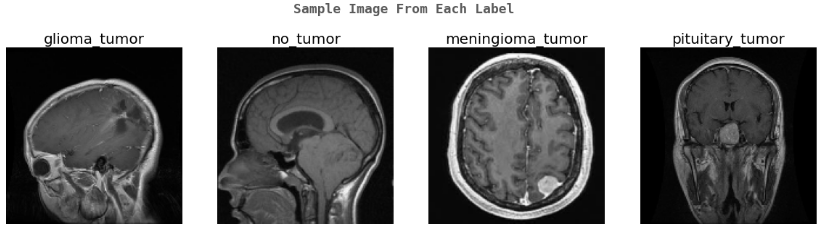
\includegraphics[scale=0.7]{Photos/dataset_sample1.PNG}
\caption{Sample Images from Dataset1} \label{fig:data_sample1}
\end{figure}

\section{Training the Model}
\subsection{Preparing the Data:}
X-train and Y-train data are prepared first so as to feed them to the model for training. X-train is an array which consists of the actual images which will be fed to the model. Y-train refers to the label about which type of tumour that particular image is. Figure \ref{fig:train_log} shows the output log of the number of images from each label being fed into the X train array. The log shows us the items/second the system was able to append to the array, based on the label; as well as the time the system takes to perform the required action on each particular label.
\begin{figure}[H]
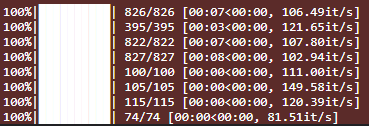
\includegraphics[scale=1]{Photos/train_log.PNG}
\caption{X train and Y train generation Log} \label{fig:train_log}
\end{figure}

\subsection{Processing the Images:}
Processing involves techniques such as cropping, RGB to Gray conversion, blurring the image and so on. This processing is performed within the web application.
Figure \ref{fig:menin_process} shows the processing results performed on meningioma tumor MRI scan.
\begin{figure}[H]
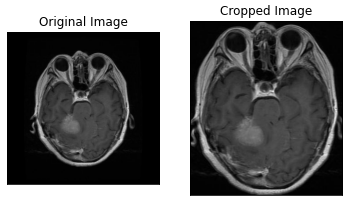
\includegraphics[scale=1]{Photos/menin_process.PNG}
\caption{Meningioma Tumor Processing Results} \label{fig:menin_process}
\end{figure}
Figure \ref{fig:glio_process} shows the processing results performed on glioma tumor MRI scan.
\begin{figure}[H]
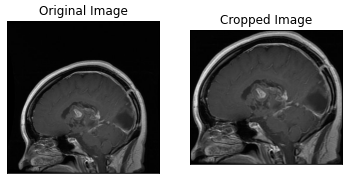
\includegraphics[scale=1]{Photos/glioma_process.png}
\caption{Glioma Tumor Processing Results} \label{fig:glio_process}
\end{figure}
Figure \ref{fig:pitu_process} shows the processing results performed on pituitary tumor MRI scan.
\begin{figure}[H]
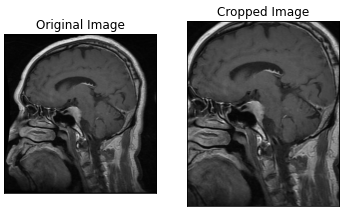
\includegraphics[scale=1]{Photos/pitu_process.PNG}
\caption{Pituitary Tumor Processing Results} \label{fig:pitu_process}
\end{figure}
Figure \ref{fig:no_process} shows the processing results performed on non tumor MRI scan.
\begin{figure}[H]
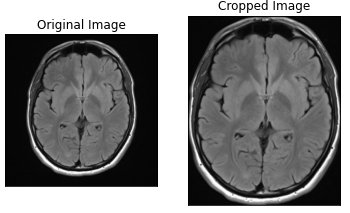
\includegraphics[scale=1]{Photos/no_process.PNG}
\caption{No Tumor Processing Results} \label{fig:no_process}
\end{figure}

\subsection{Downloading the pre-trained model:}
Once the data has been prepared, it has to be provided as input to the model. Since the project uses, transfer learning as the model defining principle, using "tf.keras.applications" we first download the model, and on top of that new training layers are added. Figure \ref{fig:model_download} shows the download log of the Densenet201 Model downloaded. The model downloaded is notop model, since on top of this model new layers have to be defined.
\begin{figure}[H]
\frame{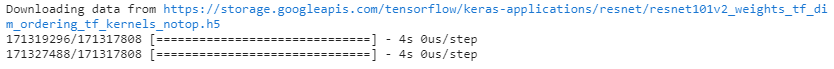
\includegraphics[scale=0.7]{Photos/model_log.PNG}}
\caption{Model Download Log} \label{fig:model_download}
\end{figure}

\subsection{Training the Model:}
Once the model has been defined, the X-Train and Y-Train data is split into a ratio of 80:10:10, where 80\% of data is train set, and 10\% data is each test and validation data set. Next, the model is compiled. It is done using model.compile function. Here the different metrics to be used/displayed are defined. This model.compile also deals with defining the optimizer to be used. Here "Adam" optimizer has been used. Once this has been done, callbacks are defined. Callbacks are the functions, which can interrupt the training of the model so as to prevent overfitting. Callbacks can also be used to keep track of the accuracy of every epoch or training cycle, and save the best model. Two callbacks have been used in the project; they are as follows
\begin{itemize}
    \item ModelCheckpoint : ModelCheckpoint callback is used to save model at particular epoch/training based on the validation accuracy or any other metric the callback is asked to check for. 
    \item ReduceLROnPlateau : ReduceLROnPlateau callback reduces the learning rate of the model when the metric stops improving.
\end{itemize}
Next, the actual parameters for training like how many iterations the model should train for, input data, callbacks and various other parameters are provided using the model.fit command. Here the model has been trained for 12 epochs. Figure \ref{fig:epoch} shows the log of the epoch training. The log shows the number of images used in each iteration, the time it took to perform the training, and the loss and accuracy metrics. 
\begin{figure}[H]
\frame{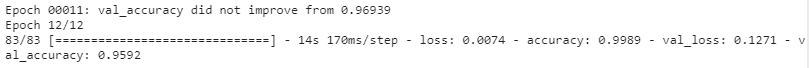
\includegraphics[scale=0.7]{Photos/epoch_.PNG}}
\caption{Epoch Log} \label{fig:epoch}
\end{figure}

\section{Training Results}
\label{section:results}
As part of model training different pre-trained models were considered. These pre-trained models are open source and are inbuilt functions of Keras.application library. 
Table \ref{tab:result} highlights the different results obtained with each version. Each version uses a different Pre-Trained model from the keras library. Due to different layers being imported in different version, the Test Accuracy and Test Loss for each version varies. Based on the results obtained, Densenet201 is the best version for the application of the project.\\
% Please add the following required packages to your document preamble:
% \usepackage{multirow}
% \usepackage{graphicx}
% \usepackage[table,xcdraw]{xcolor}
% If you use beamer only pass "xcolor=table" option, i.e. \documentclass[xcolor=table]{beamer}
% Please add the following required packages to your document preamble:
% \usepackage{multirow}
% \usepackage{graphicx}
% \usepackage[table,xcdraw]{xcolor}
% If you use beamer only pass "xcolor=table" option, i.e. \documentclass[xcolor=table]{beamer}
% Please add the following required packages to your document preamble:
% \usepackage{multirow}
% \usepackage{graphicx}
% \usepackage[table,xcdraw]{xcolor}
% If you use beamer only pass "xcolor=table" option, i.e. \documentclass[xcolor=table]{beamer}
% Please add the following required packages to your document preamble:
% \usepackage{graphicx}
% \usepackage[table,xcdraw]{xcolor}
% If you use beamer only pass "xcolor=table" option, i.e. \documentclass[xcolor=table]{beamer}
% Please add the following required packages to your document preamble:
% \usepackage{graphicx}
% \usepackage[table,xcdraw]{xcolor}
% If you use beamer only pass "xcolor=table" option, i.e. \documentclass[xcolor=table]{beamer}
\begin{table}[h!]
\caption{Results obtained from each version}
\label{tab:result}
\resizebox{14cm}{!}{%
\begin{tabular}{|c|c|c|c|}
\hline
\rowcolor[HTML]{CBCEFB} 
\multicolumn{1}{|l|}{\cellcolor[HTML]{CBCEFB}\textbf{Version}} & \textbf{Model}    & \textbf{Test Accuracy} & \textbf{Test Loss} \\ \hline
1                                                              & Densenet121       & 0.960244656         & 0.186115995            \\ \hline
2                                                              & Densenet169       & 0.966360867         & 0.16515483             \\ \hline
3                                                              & Densenet201       & 0.972477078         & 0.142509162            \\ \hline
4                                                              & EfficientNetB0    & 0.788990855         & 0.551147401            \\ \hline
5                                                              & EfficientNetB1    & 0.440366983         & 2.732621908            \\ \hline
6                                                              & EfficientNetB2    & 0.773700297         & 0.561737001            \\ \hline
7                                                              & EfficientNetB3    & 0.65749234          & 1.091159701            \\ \hline
8                                                              & EfficientNetB4    & 0.76452601          & 0.656704843            \\ \hline
9                                                              & EfficientNetB5    & 0.409785926         & 3.710002422            \\ \hline
10                                                             & EfficientNetB6    & 0.865443408         & 0.362860888            \\ \hline
11                                                             & EfficientNetB7    & 0.446483195         & 2.516769886            \\ \hline
12                                                             & InceptionResNetV2 & 0.960244656         & 0.217766672            \\ \hline
13                                                             & InceptionV3       & 0.963302732         & 0.139801413            \\ \hline
14                                                             & MobileNet         & 0.966360867         & 0.169000089            \\ \hline
15                                                             & MobileNetV2       & 0.926605523         & 0.51417464             \\ \hline
16                                                             & MobileNetV3Large  & 0.840978622         & 0.996828198            \\ \hline
17                                                             & MobileNetV3Small  & 0.85015291          & 0.87231195             \\ \hline
18                                                             & ResNet101         & 0.948012233         & 0.204600975            \\ \hline
19                                                             & ResNet101V2       & 0.929663599         & 0.251542419            \\ \hline
\end{tabular}%
}
\end{table}

\section{Results of the Best Version}
Based on the results obtained from table \ref{tab:result} Densenet201 proves to be the best model for the problem the project aims to solve. Figure \ref{fig:best_version} shows the accuracy and loss graph of the model trained using Densenet201 as base layers.
\begin{figure}[H]
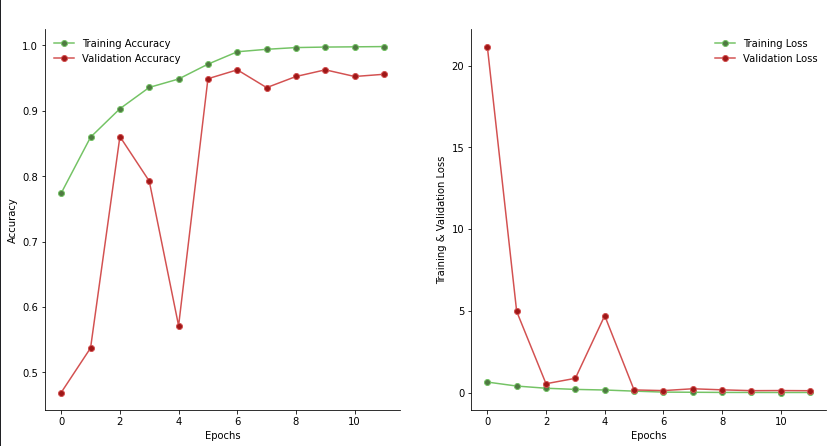
\includegraphics[scale=0.6]{Photos/accuracy_loss.PNG}
\caption{Accuracy Graph from the best version} \label{fig:best_version}
\end{figure}
Figure \ref{fig:confusion} shows the confusion matrix heatmap of the Densenet201 model. Confusion matrix is an evaluation parameter which gives an insight into the model accuracy by comparing the actual and predicted outputs with each other. As it can be observed, the model has a very high accuracy and is able to correctly classify images into their correct class.
\begin{figure}[H]
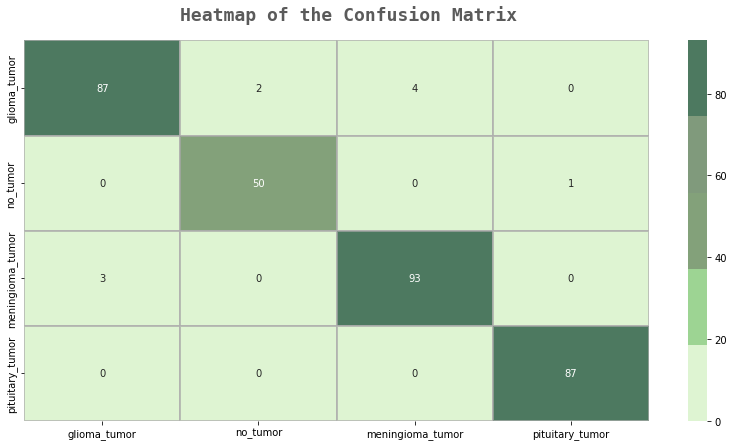
\includegraphics[scale=0.6]{Photos/confusion_matrix.PNG}
\caption{Confusion Matrix} \label{fig:confusion}
\end{figure}
Figure shows the classification report. A classification report, gives information about the quality of the predictions. There are factors like, precision, recall, f1-score and accuracy. The numbers 0,1,2, and 3 are the numbers of the labels, in order of glioma, no-tumor, meningioma and pituitary tumor. T
\begin{figure}[H]
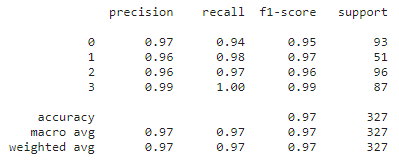
\includegraphics[scale=1.3]{Photos/class_report.PNG}
\caption{Classification Report} \label{fig:class_report}
\end{figure}

\section{Accuracy and Loss graph of every version in table \ref{tab:result}}
Figure \ref{fig:dense121} shows the test loss vs epochs and test accuracy vs epoch graph of the model generated using Densenet121 as the base model.
\begin{figure}[H]
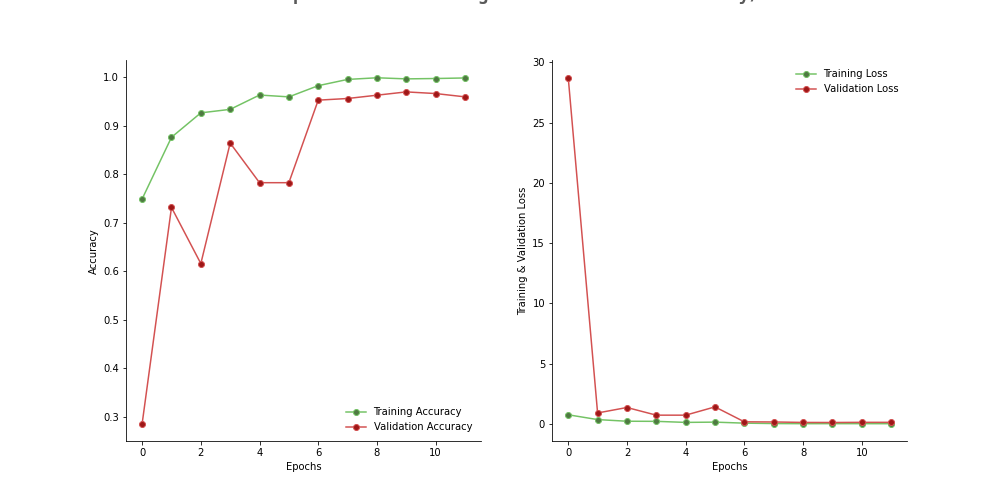
\includegraphics[scale=0.44]{Photos/densenet121_plot.png}
\caption{Version 1 : Densenet121} \label{fig:dense121}
\end{figure}
Figure \ref{fig:dense169} shows the test loss vs epochs and test accuracy vs epoch graph of the model generated using Densenet169 as the base model.
\begin{figure}[H]
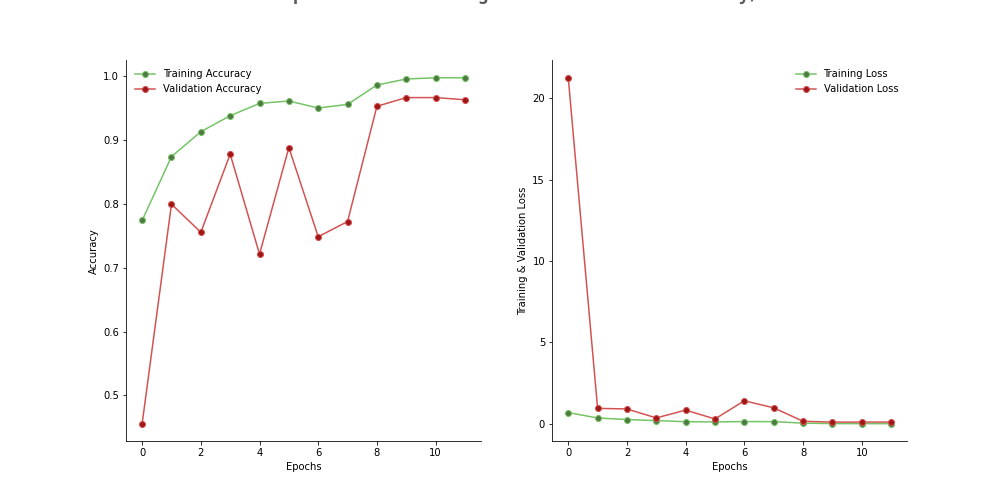
\includegraphics[scale=0.3]{Photos/densenet169_plot.png}
\caption{Version 2 : Densenet169} \label{fig:dense169}
\end{figure}
Figure \ref{fig:dense201} shows the test loss vs epochs and test accuracy vs epoch graph of the model generated using Densenet201 as the base model.
\begin{figure}[H]
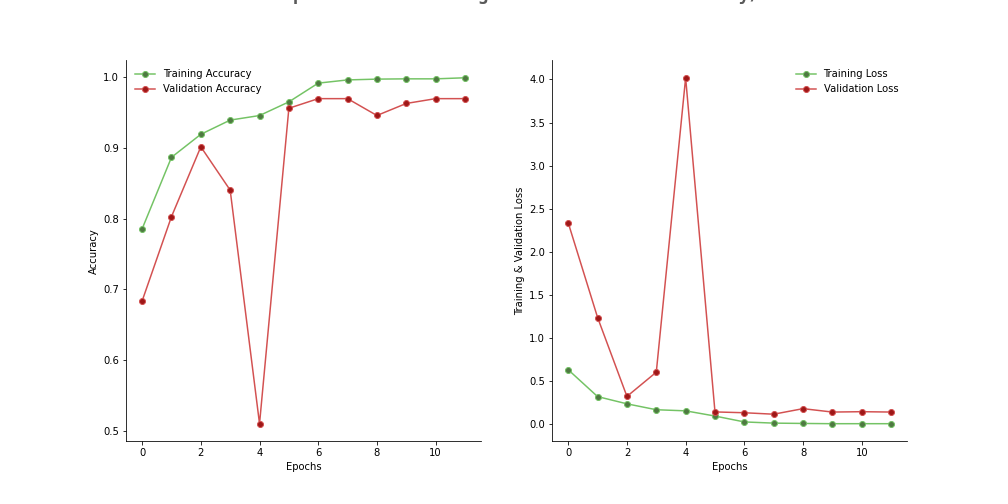
\includegraphics[scale=0.29]{Photos/densenet201_plot.png}
\caption{Version 3 : Densenet201} \label{fig:dense201}
\end{figure}
Figure \ref{fig:effnetb0} shows the test loss vs epochs and test accuracy vs epoch graph of the model generated using EfficientNetB0 as the base model.
\begin{figure}[H]
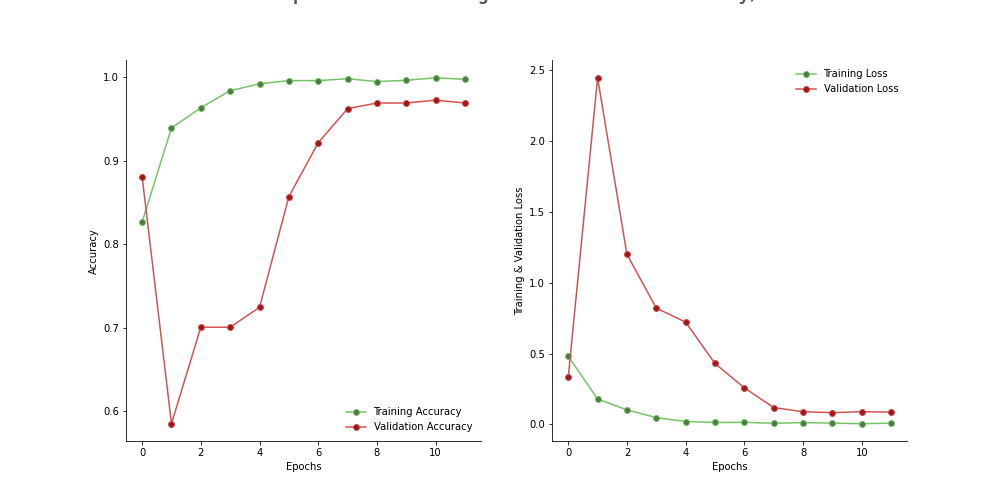
\includegraphics[scale=0.29]{Photos/EfficientNetB0_plot.png}
\caption{Version 4 : EfficientNetB0} \label{fig:effnetb0}
\end{figure}
Figure \ref{fig:effnetb1} shows the test loss vs epochs and test accuracy vs epoch graph of the model generated using EfficientNetB1 as the base model.
\begin{figure}[H]
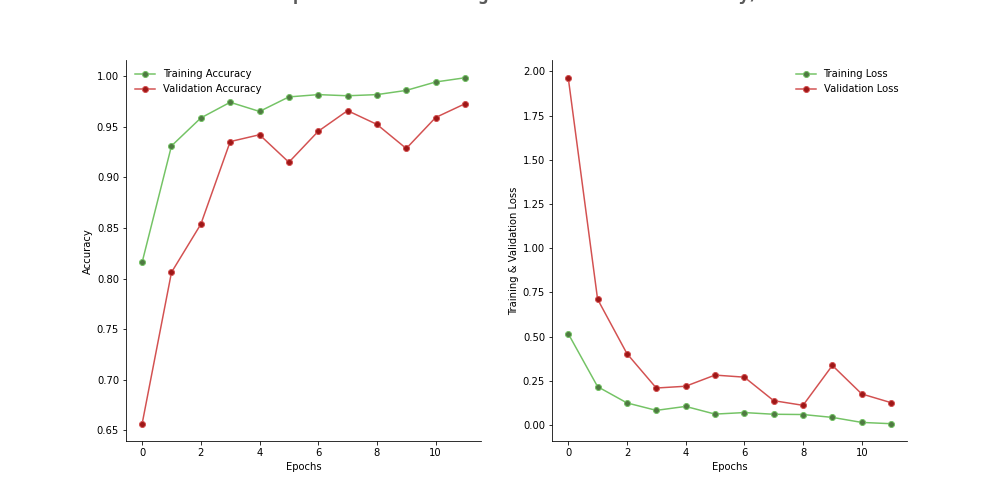
\includegraphics[scale=0.29]{Photos/EfficientNetB1_plot.png}
\caption{Version 5 : EfficientNetB1} \label{fig:effnetb1}
\end{figure}
Figure \ref{fig:effnetb2} shows the test loss vs epochs and test accuracy vs epoch graph of the model generated using EfficientNetB2 as the base model.
\begin{figure}[H]
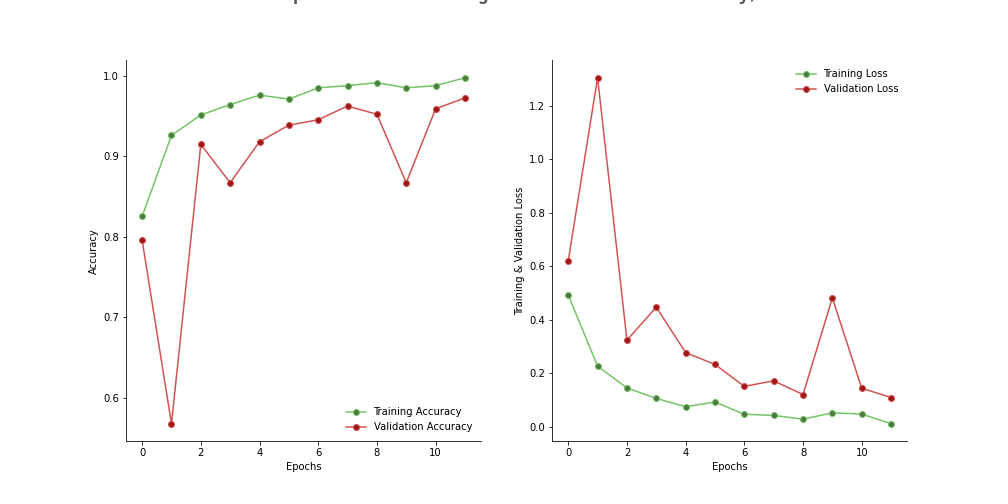
\includegraphics[scale=0.29]{Photos/EfficientNetB2_plot.png}
\caption{Version 6 : EfficientNetB2} \label{fig:effnetb2}
\end{figure}
Figure \ref{fig:effnetb3} shows the test loss vs epochs and test accuracy vs epoch graph of the model generated using EfficientNetB3 as the base model.
\begin{figure}[H]
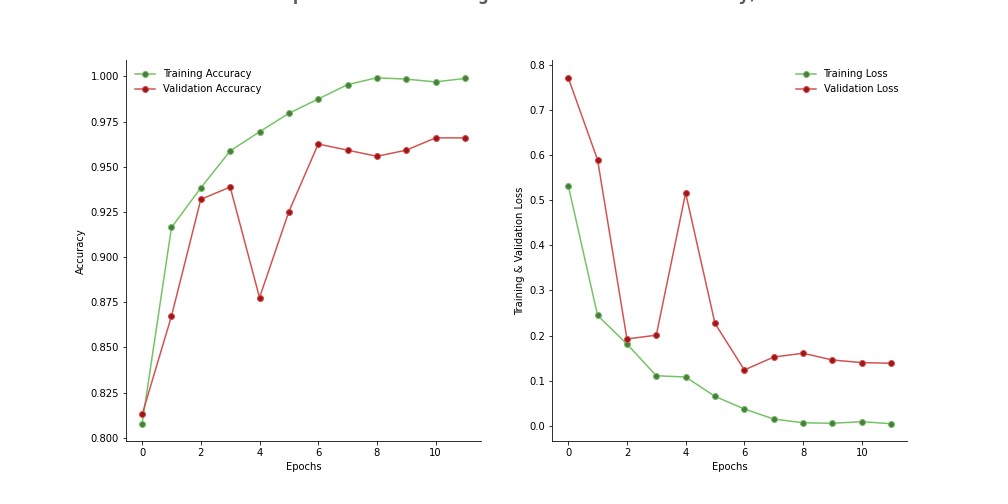
\includegraphics[scale=0.29]{Photos/EfficientNetB3_plot.png}
\caption{Version 7 : EfficientNetB3} \label{fig:effnetb3}
\end{figure}
Figure \ref{fig:effnetb4} shows the test loss vs epochs and test accuracy vs epoch graph of the model generated using EfficientNetB4 as the base model.
\begin{figure}[H]
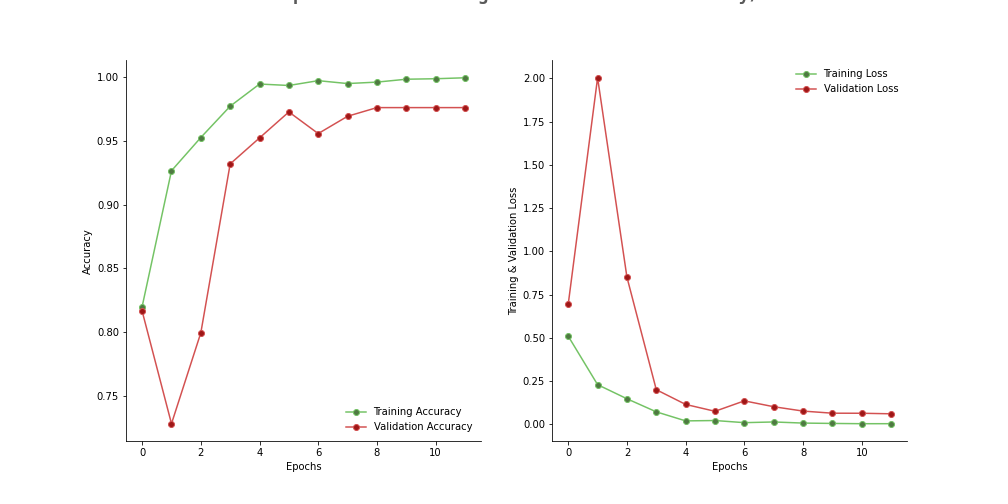
\includegraphics[scale=0.29]{Photos/EfficientNetB4_plot.png}
\caption{Version 8 : EfficientNetB4} \label{fig:effnetb4}
\end{figure}
Figure \ref{fig:effnetb5} shows the test loss vs epochs and test accuracy vs epoch graph of the model generated using EfficientNetB5 as the base model.
\begin{figure}[H]
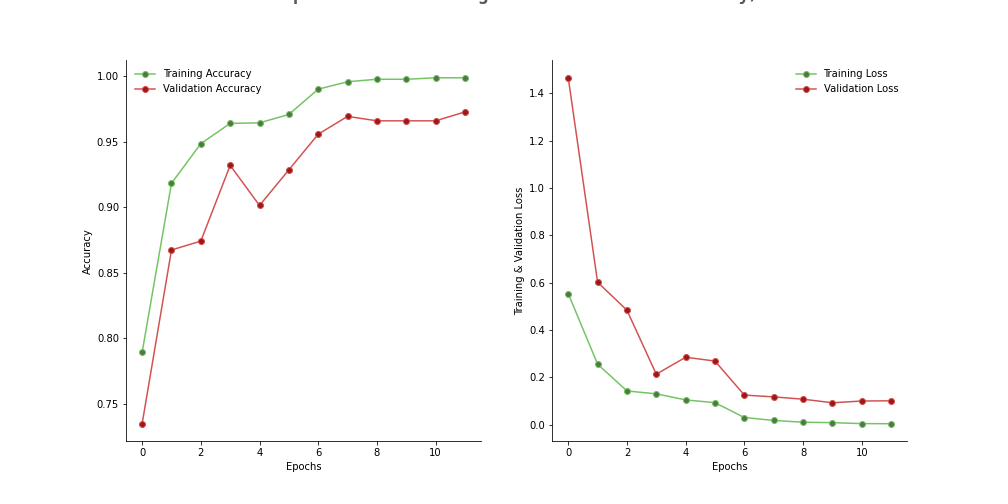
\includegraphics[scale=0.29]{Photos/EfficientNetB5_plot.png}
\caption{Version 9 : EfficientNetB5} \label{fig:effnetb5}
\end{figure}
Figure \ref{fig:effnetb6} shows the test loss vs epochs and test accuracy vs epoch graph of the model generated using EfficientNetB6 as the base model.
\begin{figure}[H]
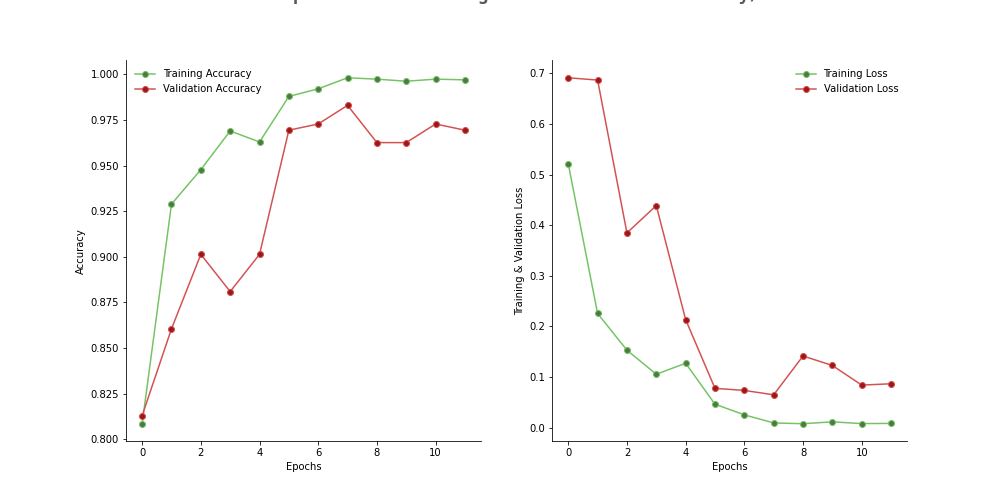
\includegraphics[scale=0.29]{Photos/EfficientNetB6_plot.png}
\caption{Version 10 : EfficientNetB6} \label{fig:effnetb6}
\end{figure}
Figure \ref{fig:effnetb7} shows the test loss vs epochs and test accuracy vs epoch graph of the model generated using EfficientNetB7 as the base model.
\begin{figure}[H]
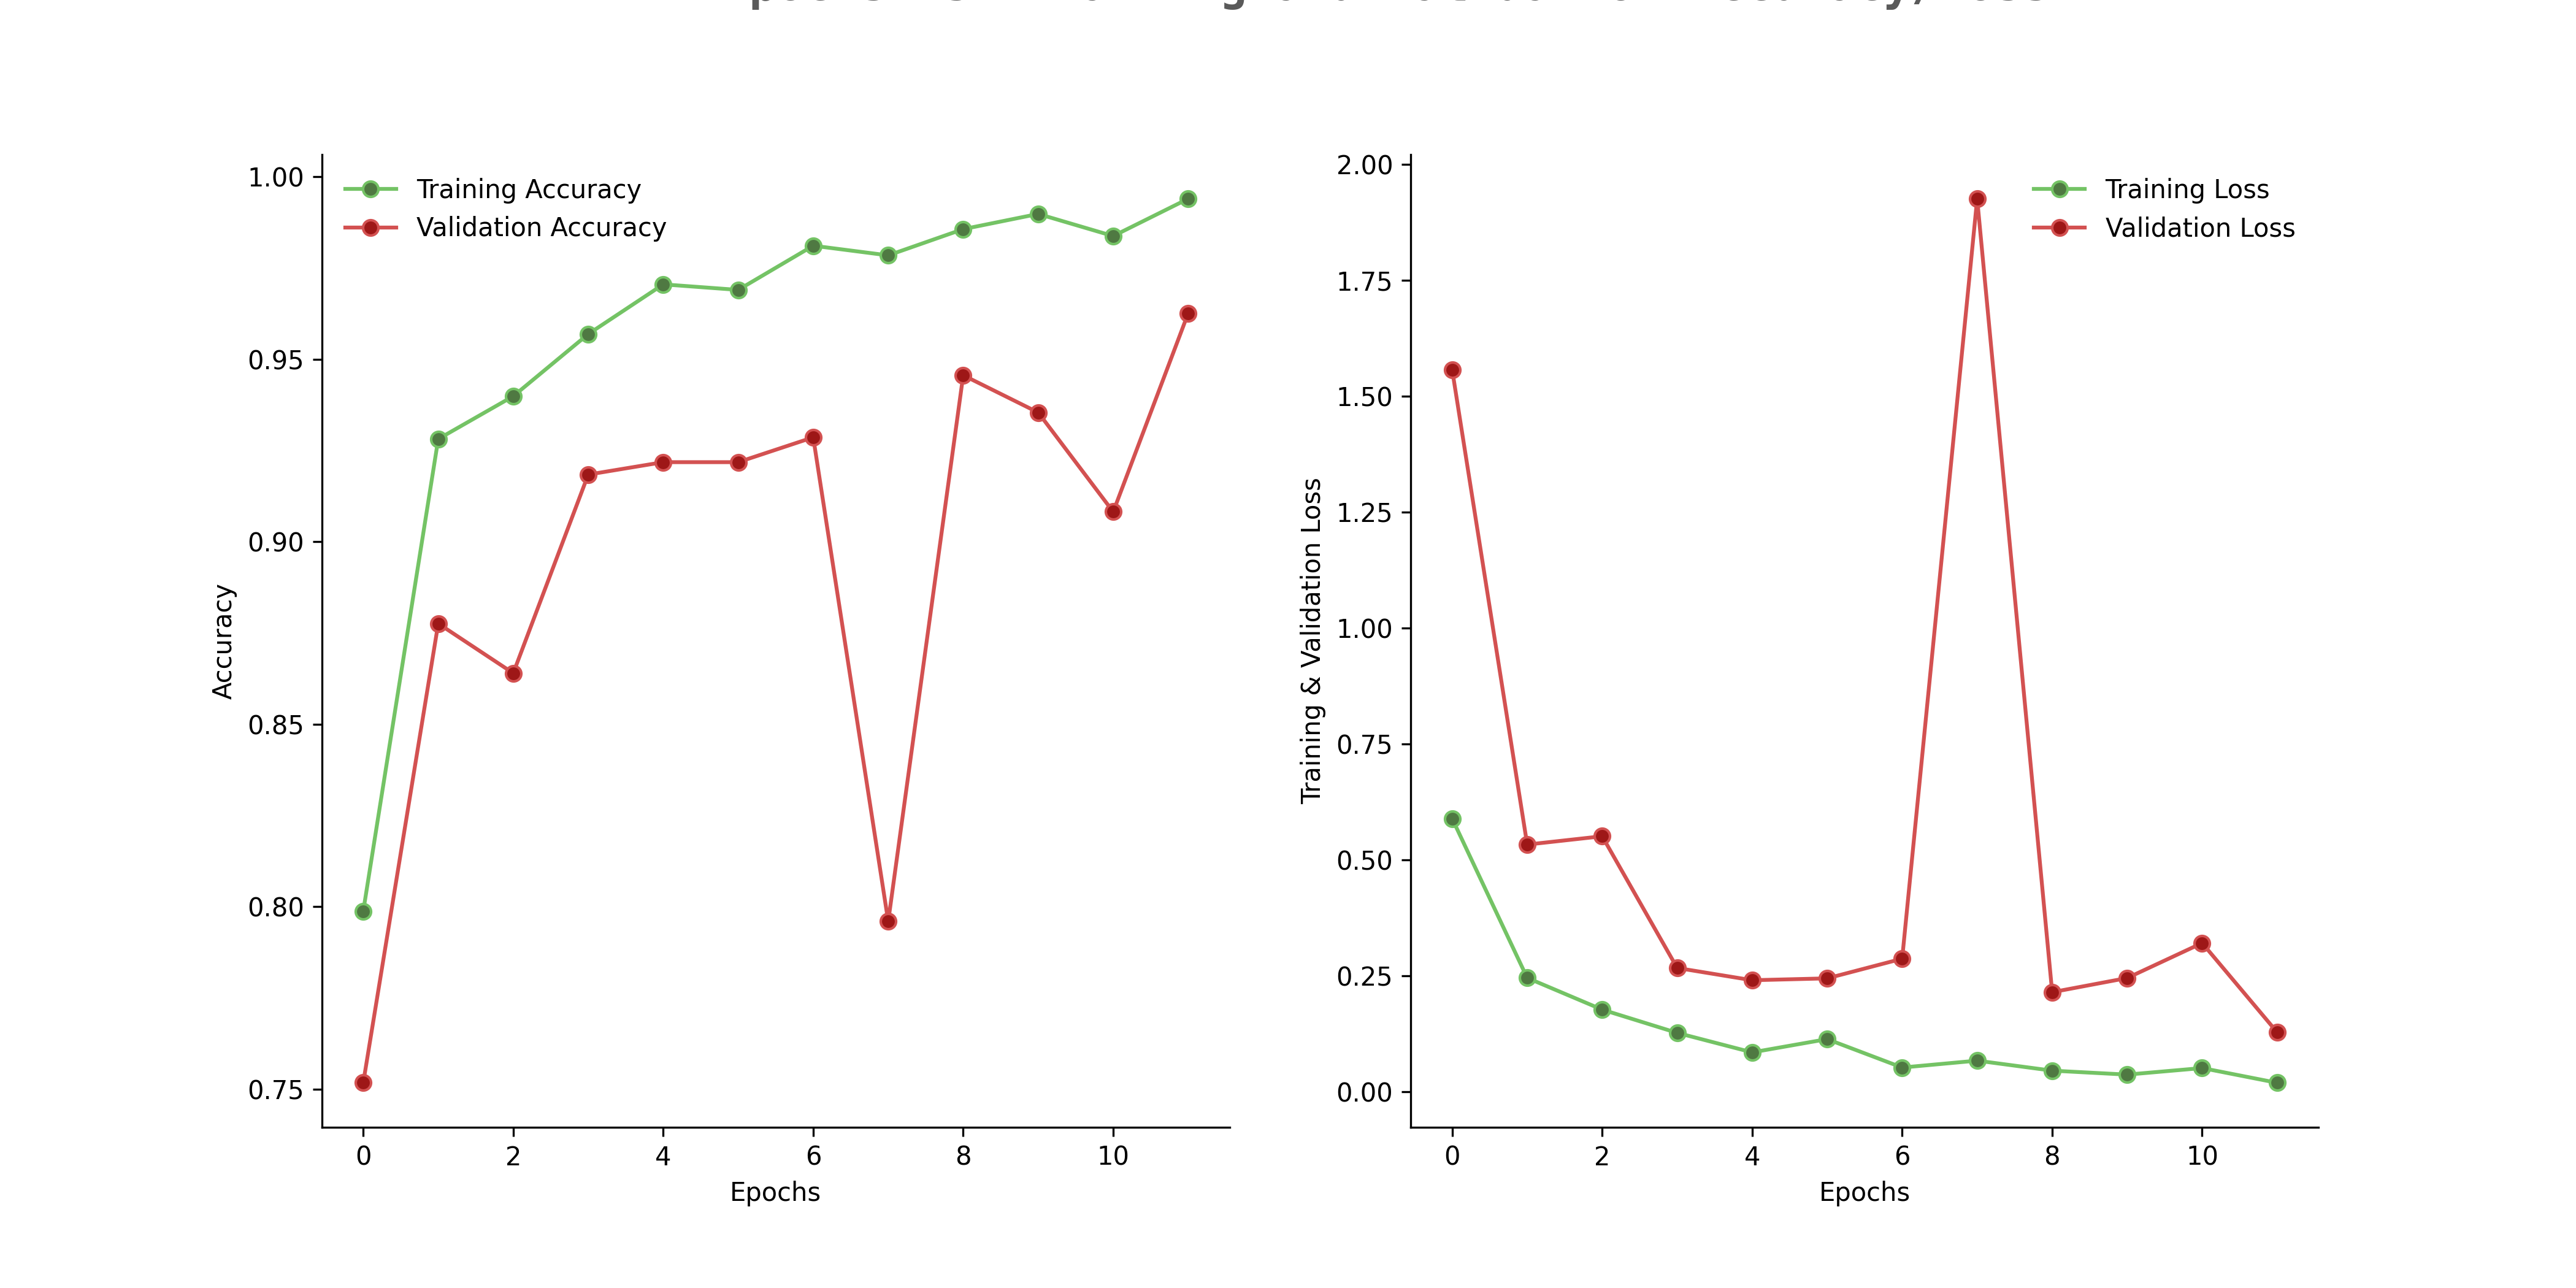
\includegraphics[scale=0.29]{Photos/EfficientNetB7_plot.png}
\caption{Version 11 : EfficientNetB7} \label{fig:effnetb7}
\end{figure}
Figure \ref{fig:inceptionresv2} shows the test loss vs epochs and test accuracy vs epoch graph of the model generated using InceptionResNetV2 as the base model.
\begin{figure}[H]
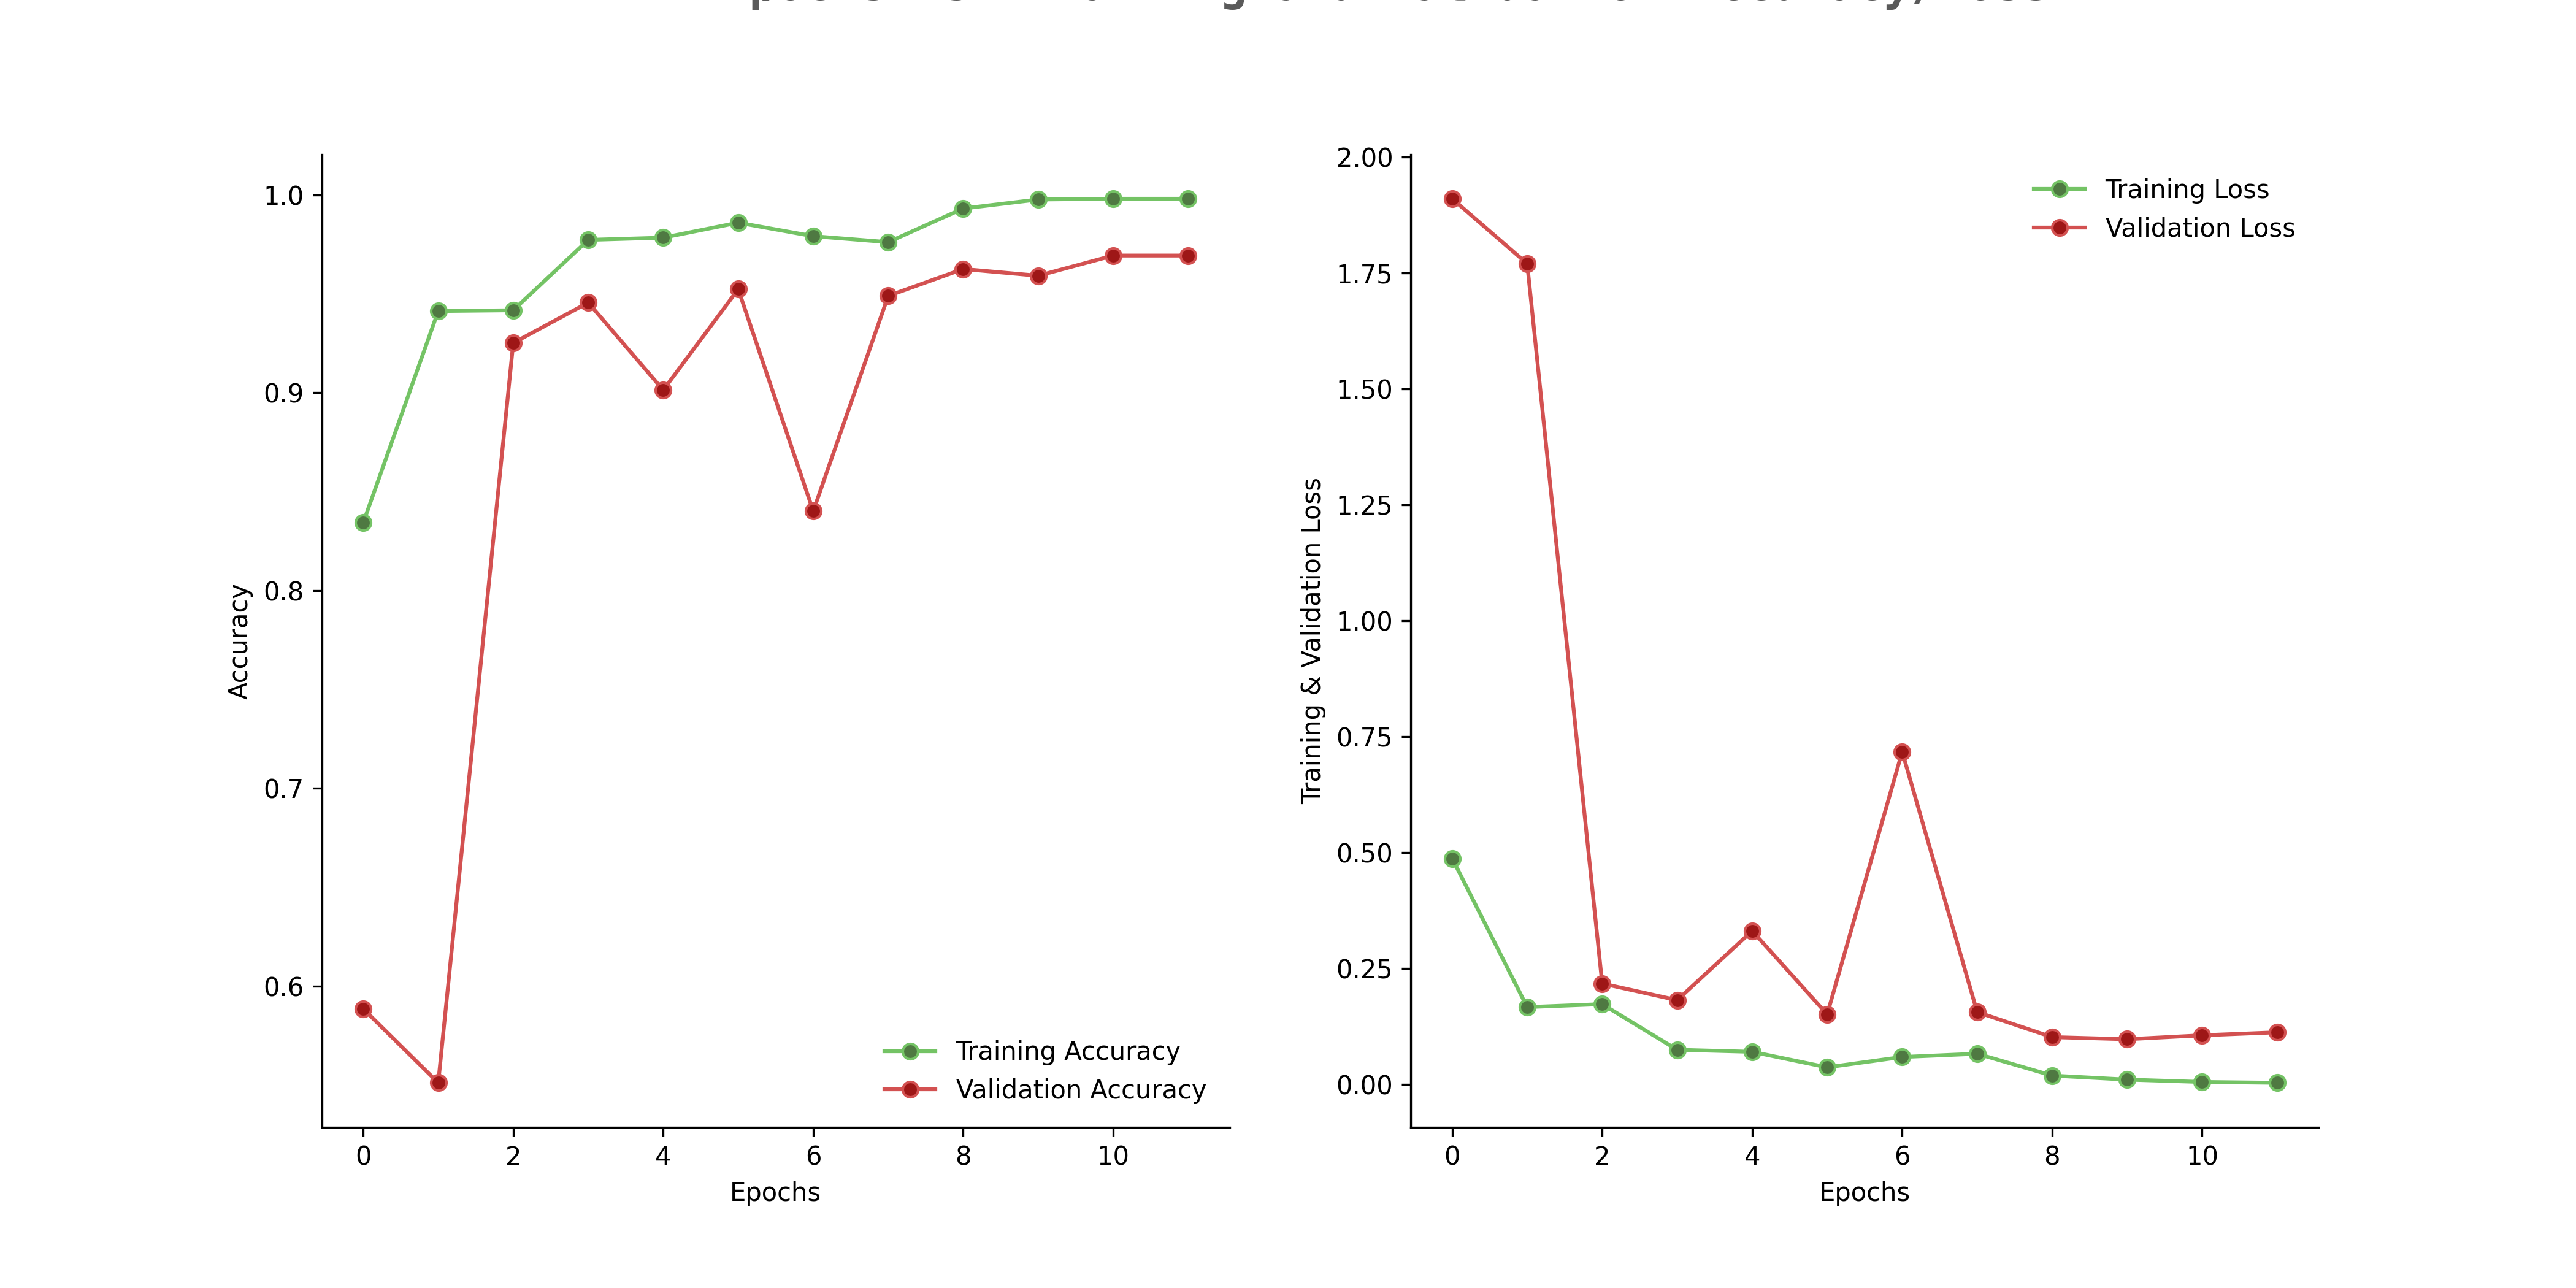
\includegraphics[scale=0.29]{Photos/InceptionResNetV2_plot.png}
\caption{Version 12 : InceptionResNetV2} \label{fig:inceptionresv2}
\end{figure}
Figure \ref{fig:inceptionv3} shows the test loss vs epochs and test accuracy vs epoch graph of the model generated using InceptionV3 as the base model.
\begin{figure}[H]
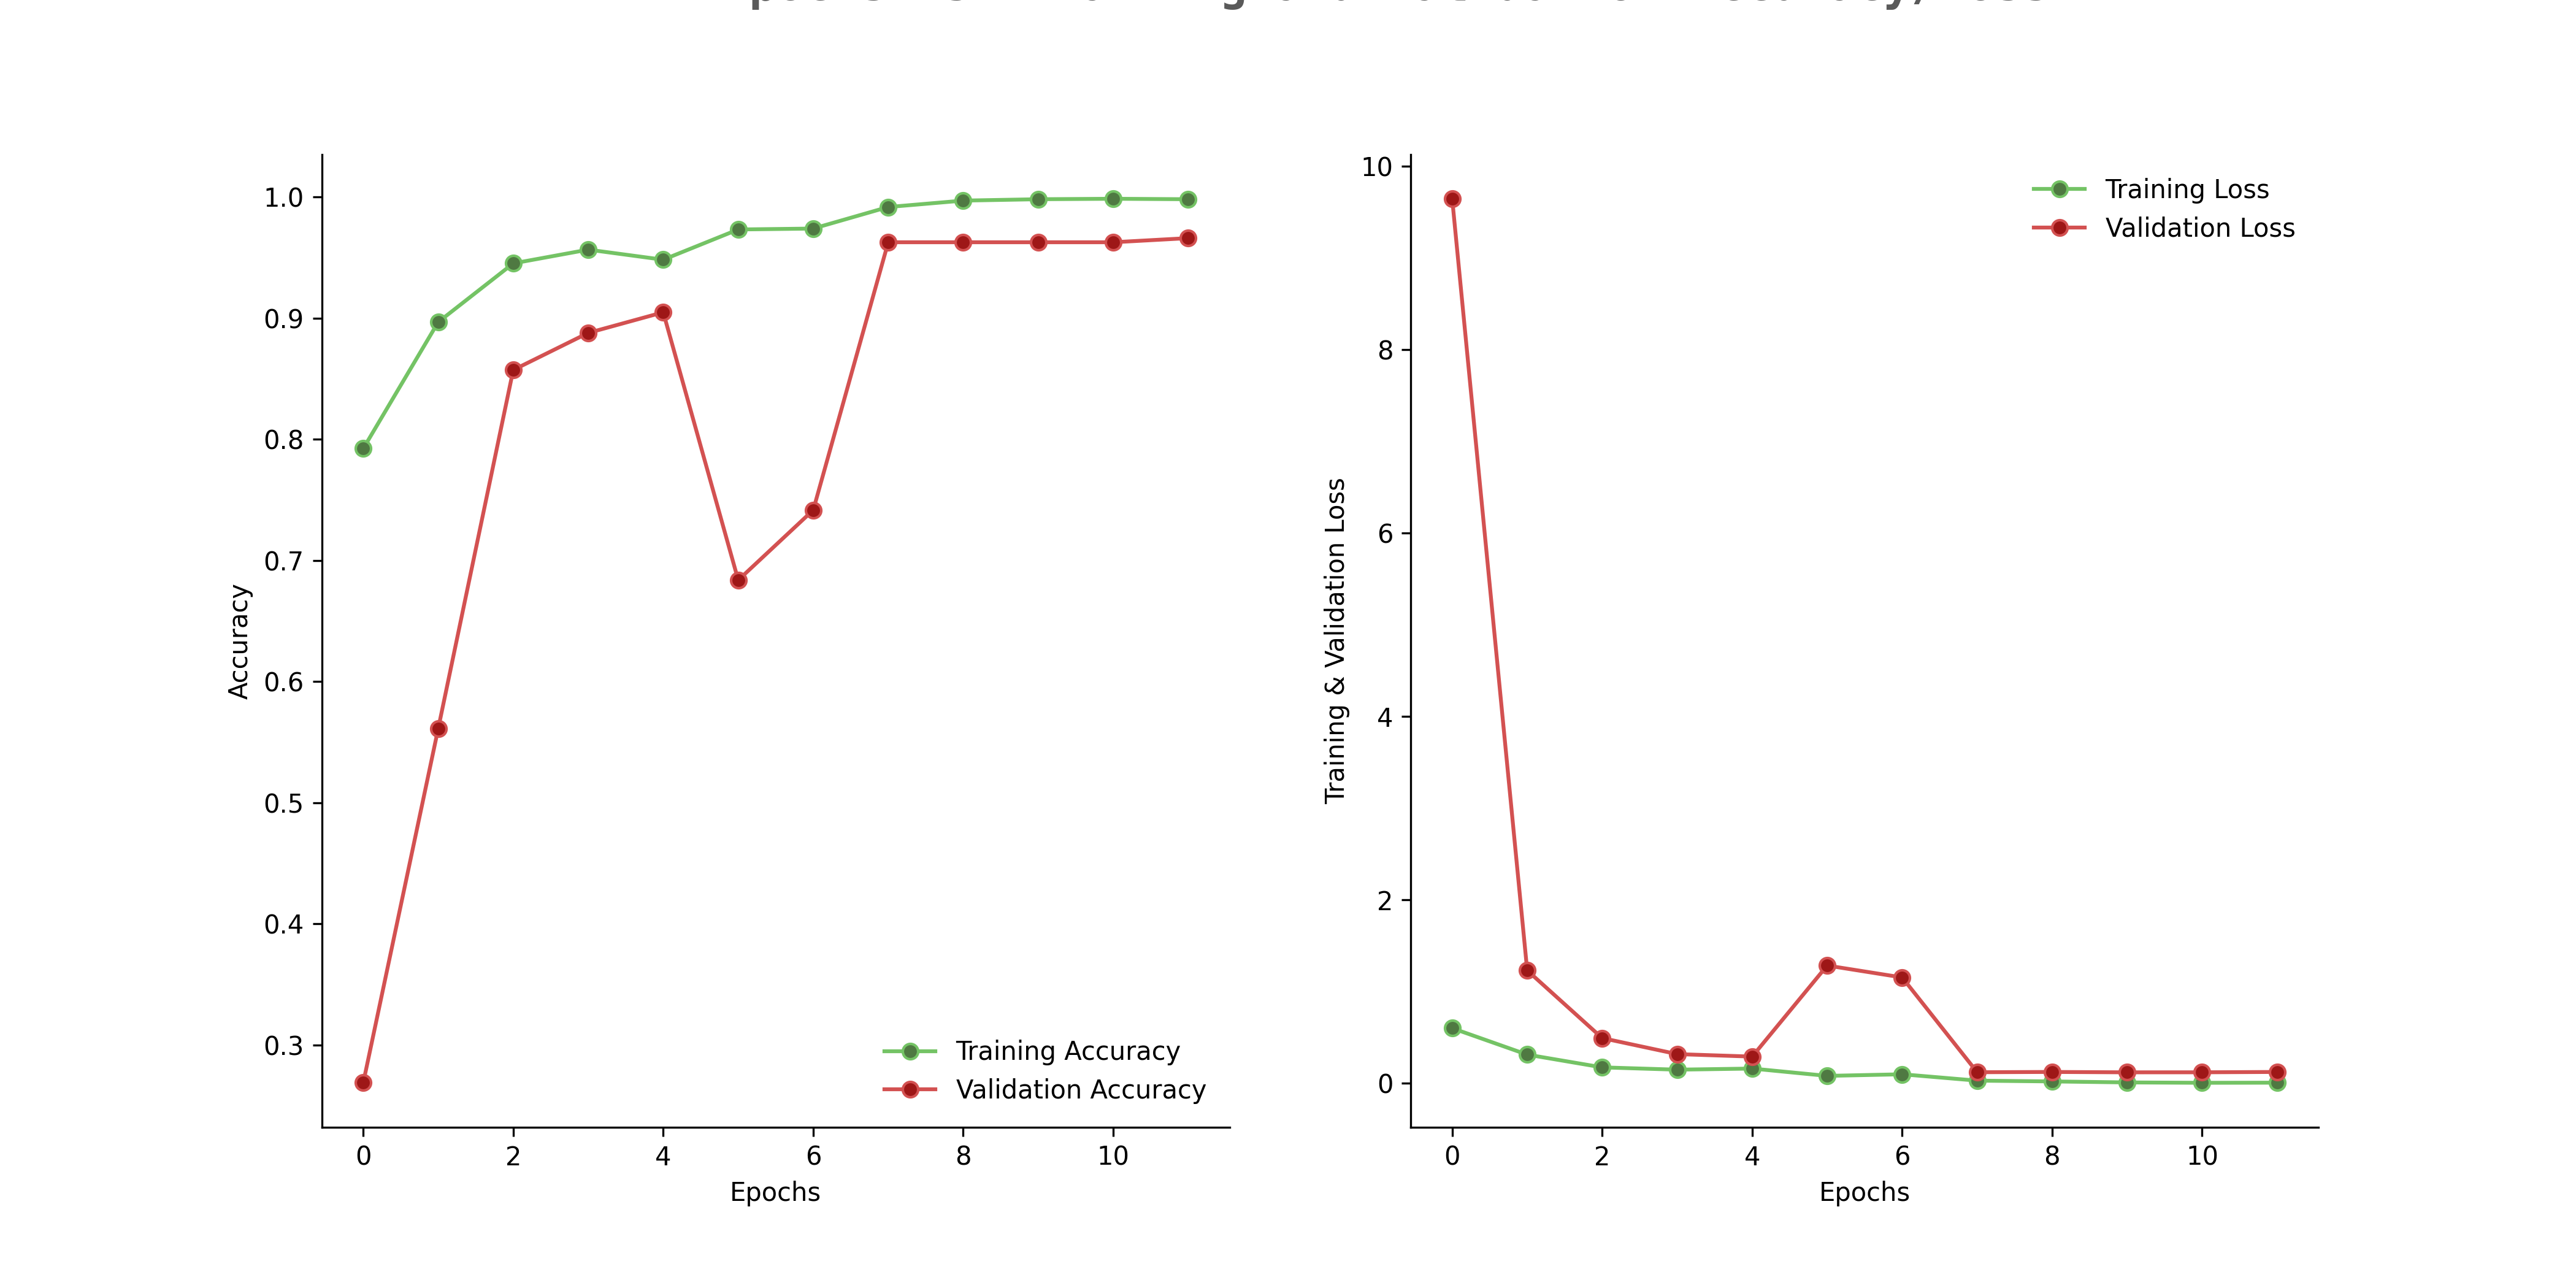
\includegraphics[scale=0.29]{Photos/InceptionV3_plot.png}
\caption{Version 13 : InceptionV3} \label{fig:inceptionv3}
\end{figure}
Figure \ref{fig:mnet} shows the test loss vs epochs and test accuracy vs epoch graph of the model generated using MobileNet as the base model.
\begin{figure}[H]
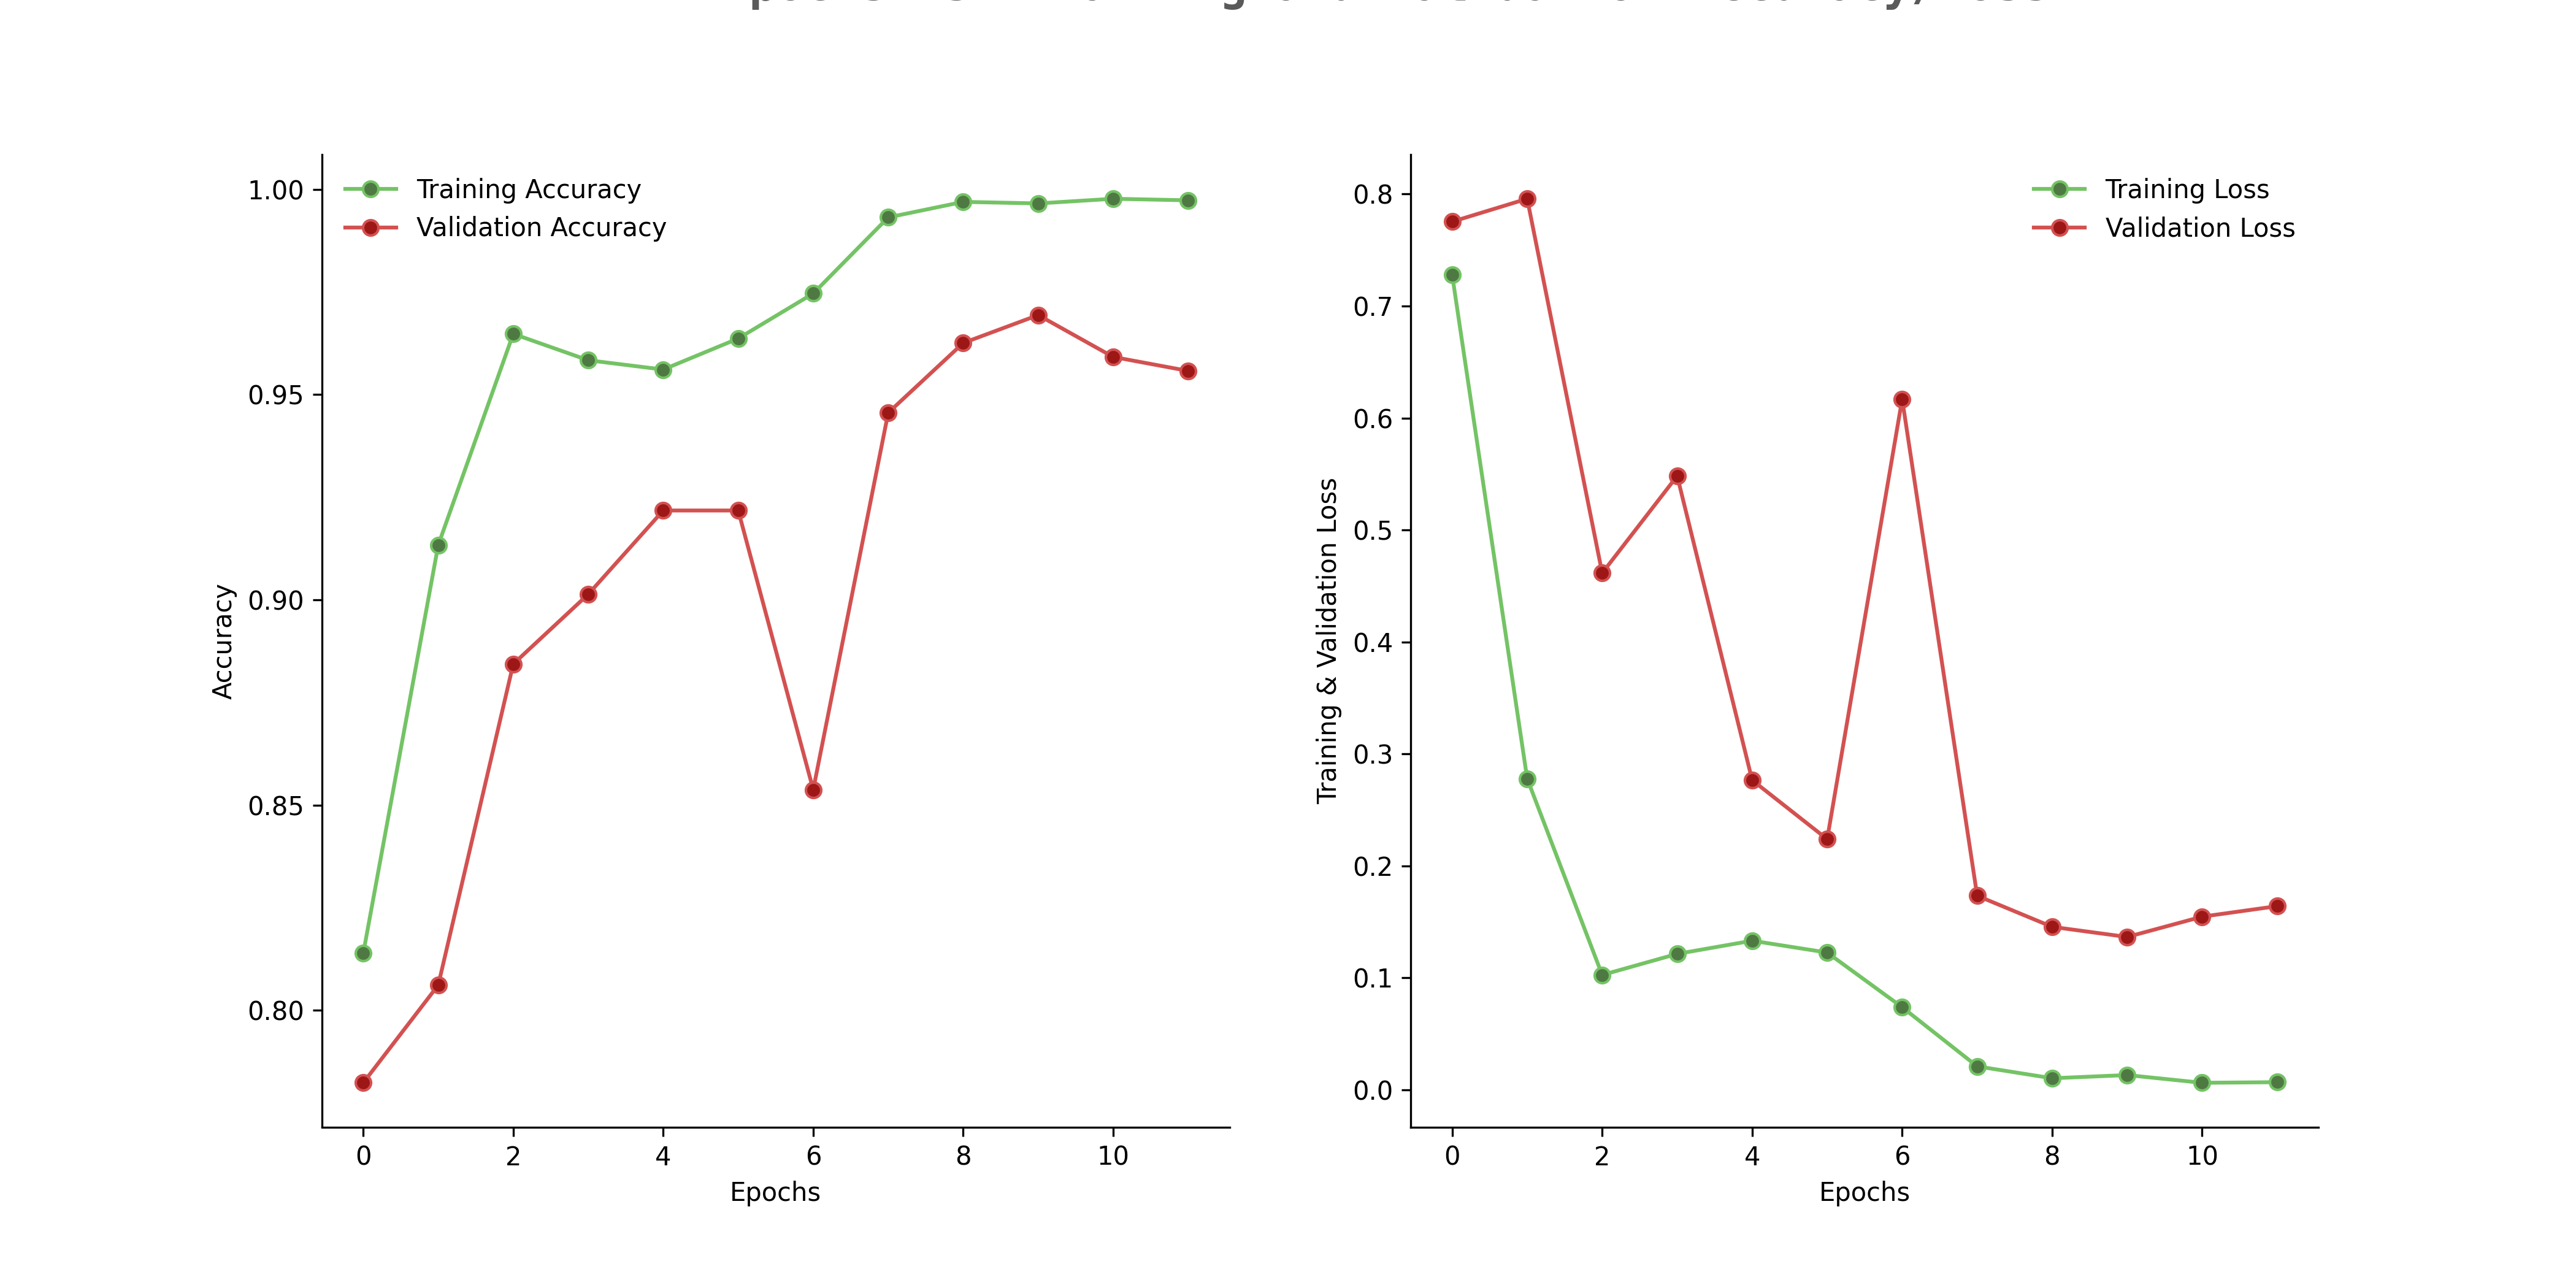
\includegraphics[scale=0.29]{Photos/MobileNet_plot.png}
\caption{Version 14 : MobileNet} \label{fig:mnet}
\end{figure}
Figure \ref{fig:mnetv2} shows the test loss vs epochs and test accuracy vs epoch graph of the model generated using MobileNetV2 as the base model.
\begin{figure}[H]
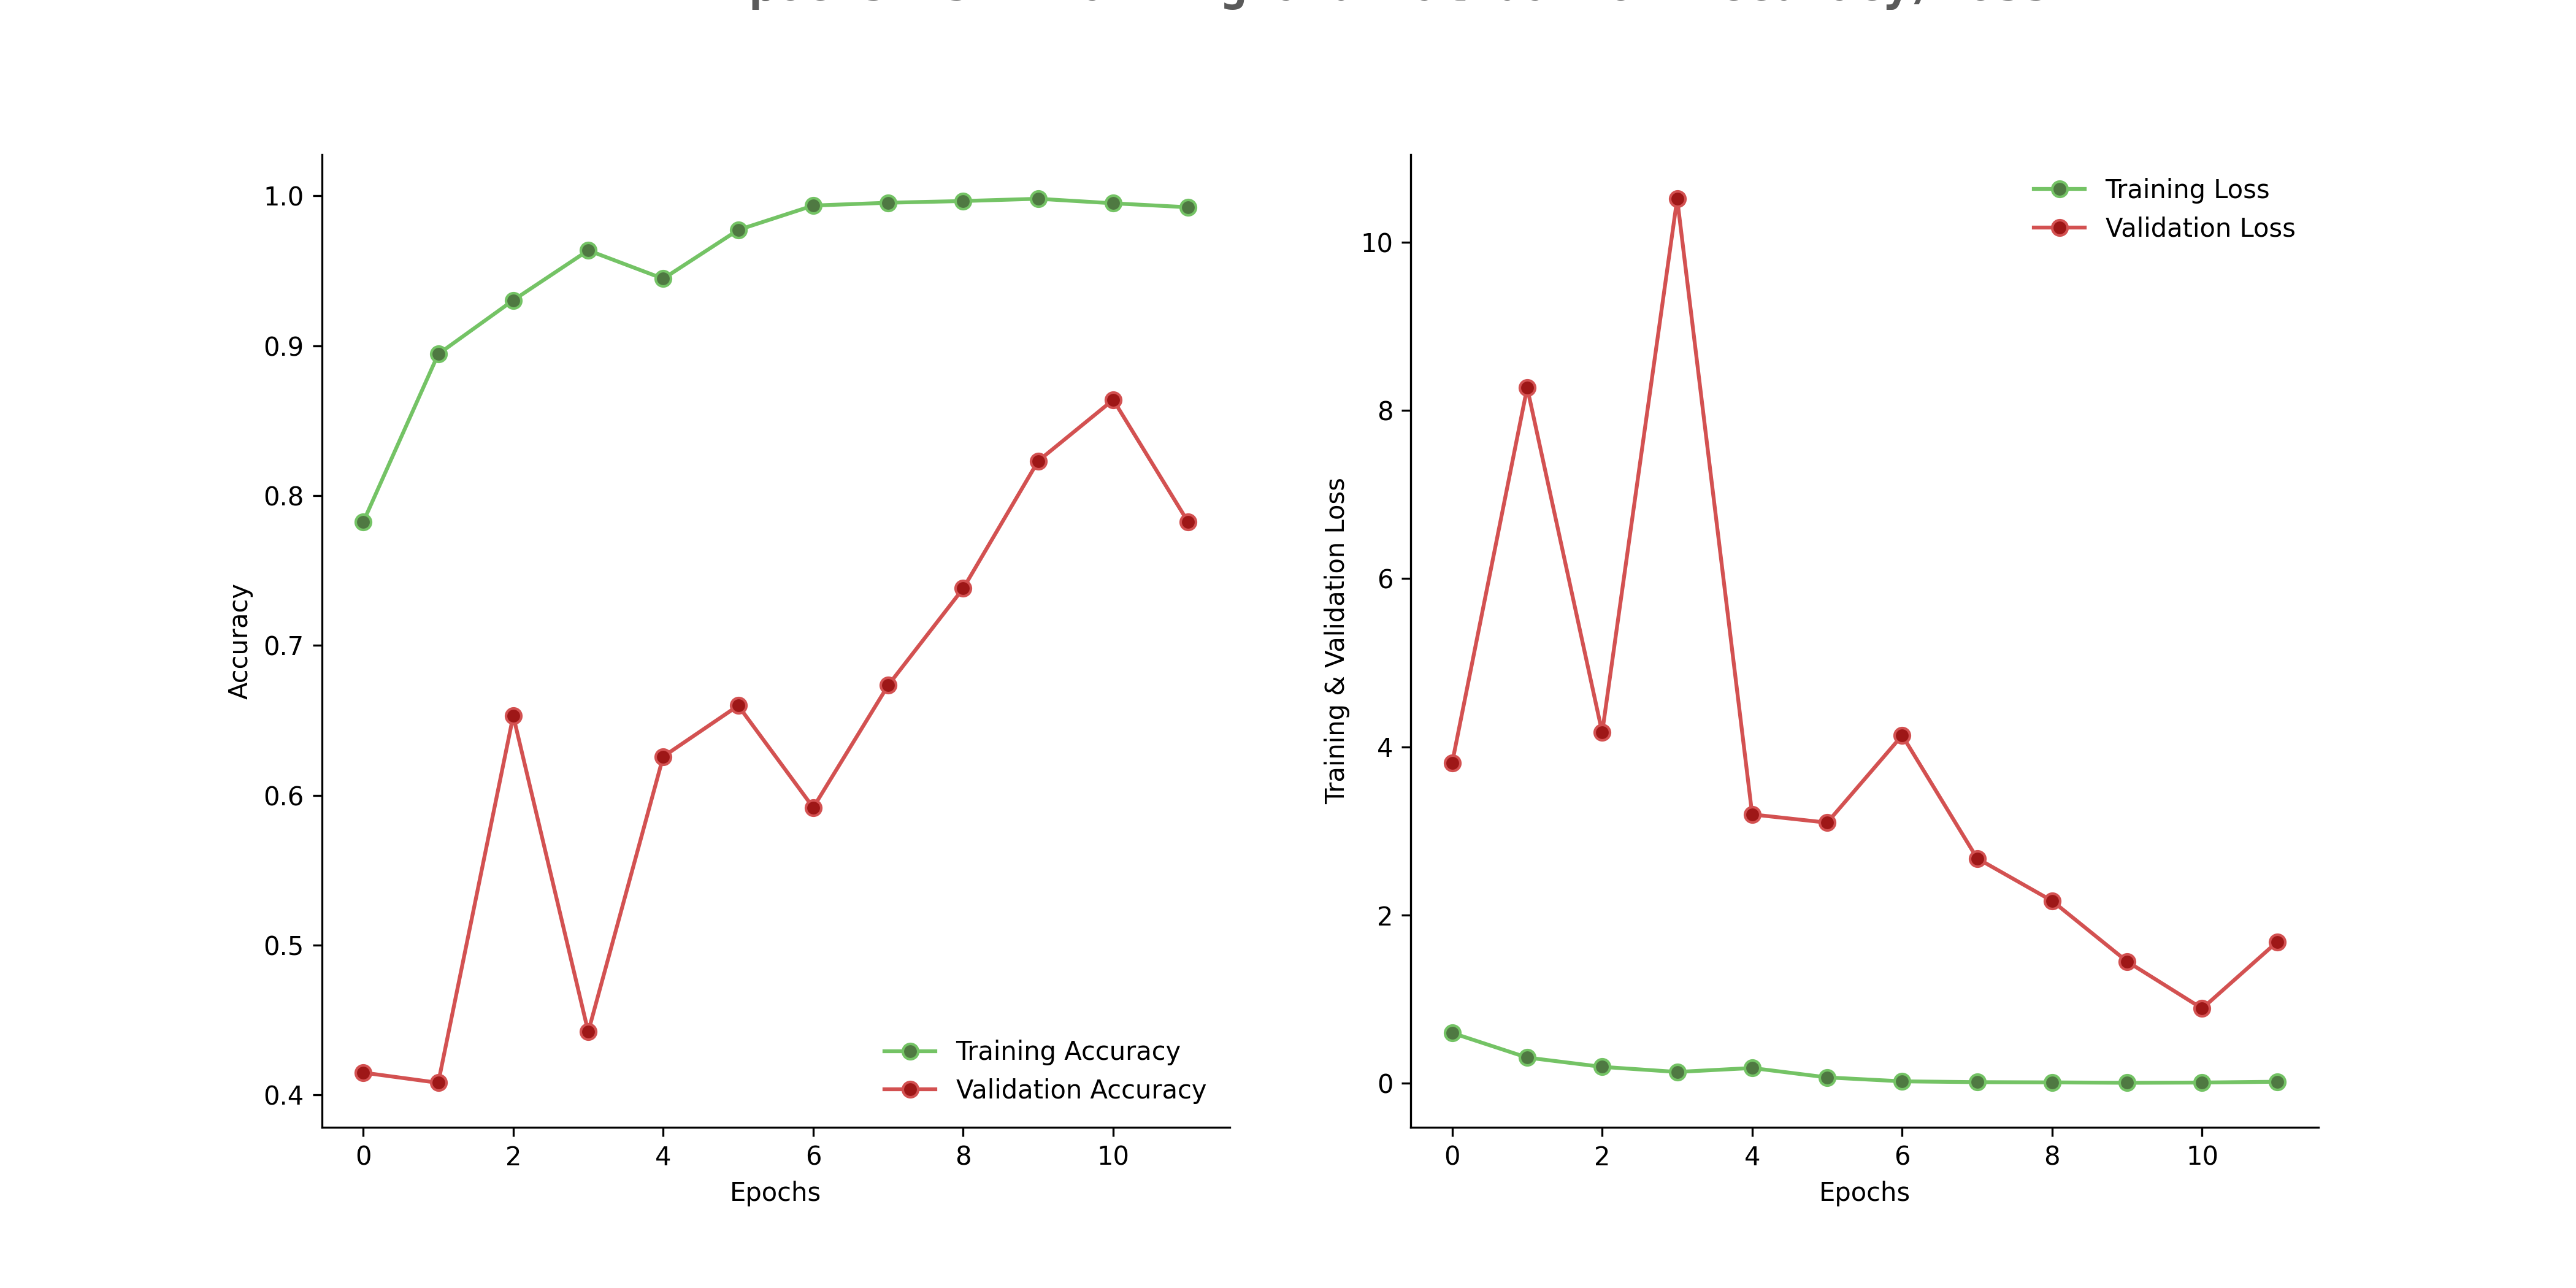
\includegraphics[scale=0.29]{Photos/MobileNetV2_plot.png}
\caption{Version 15 : MobileNetV2} \label{fig:mnetv2}
\end{figure}
Figure \ref{fig:mnetv3l} shows the test loss vs epochs and test accuracy vs epoch graph of the model generated using MobileNetV3Large as the base model.
\begin{figure}[H]
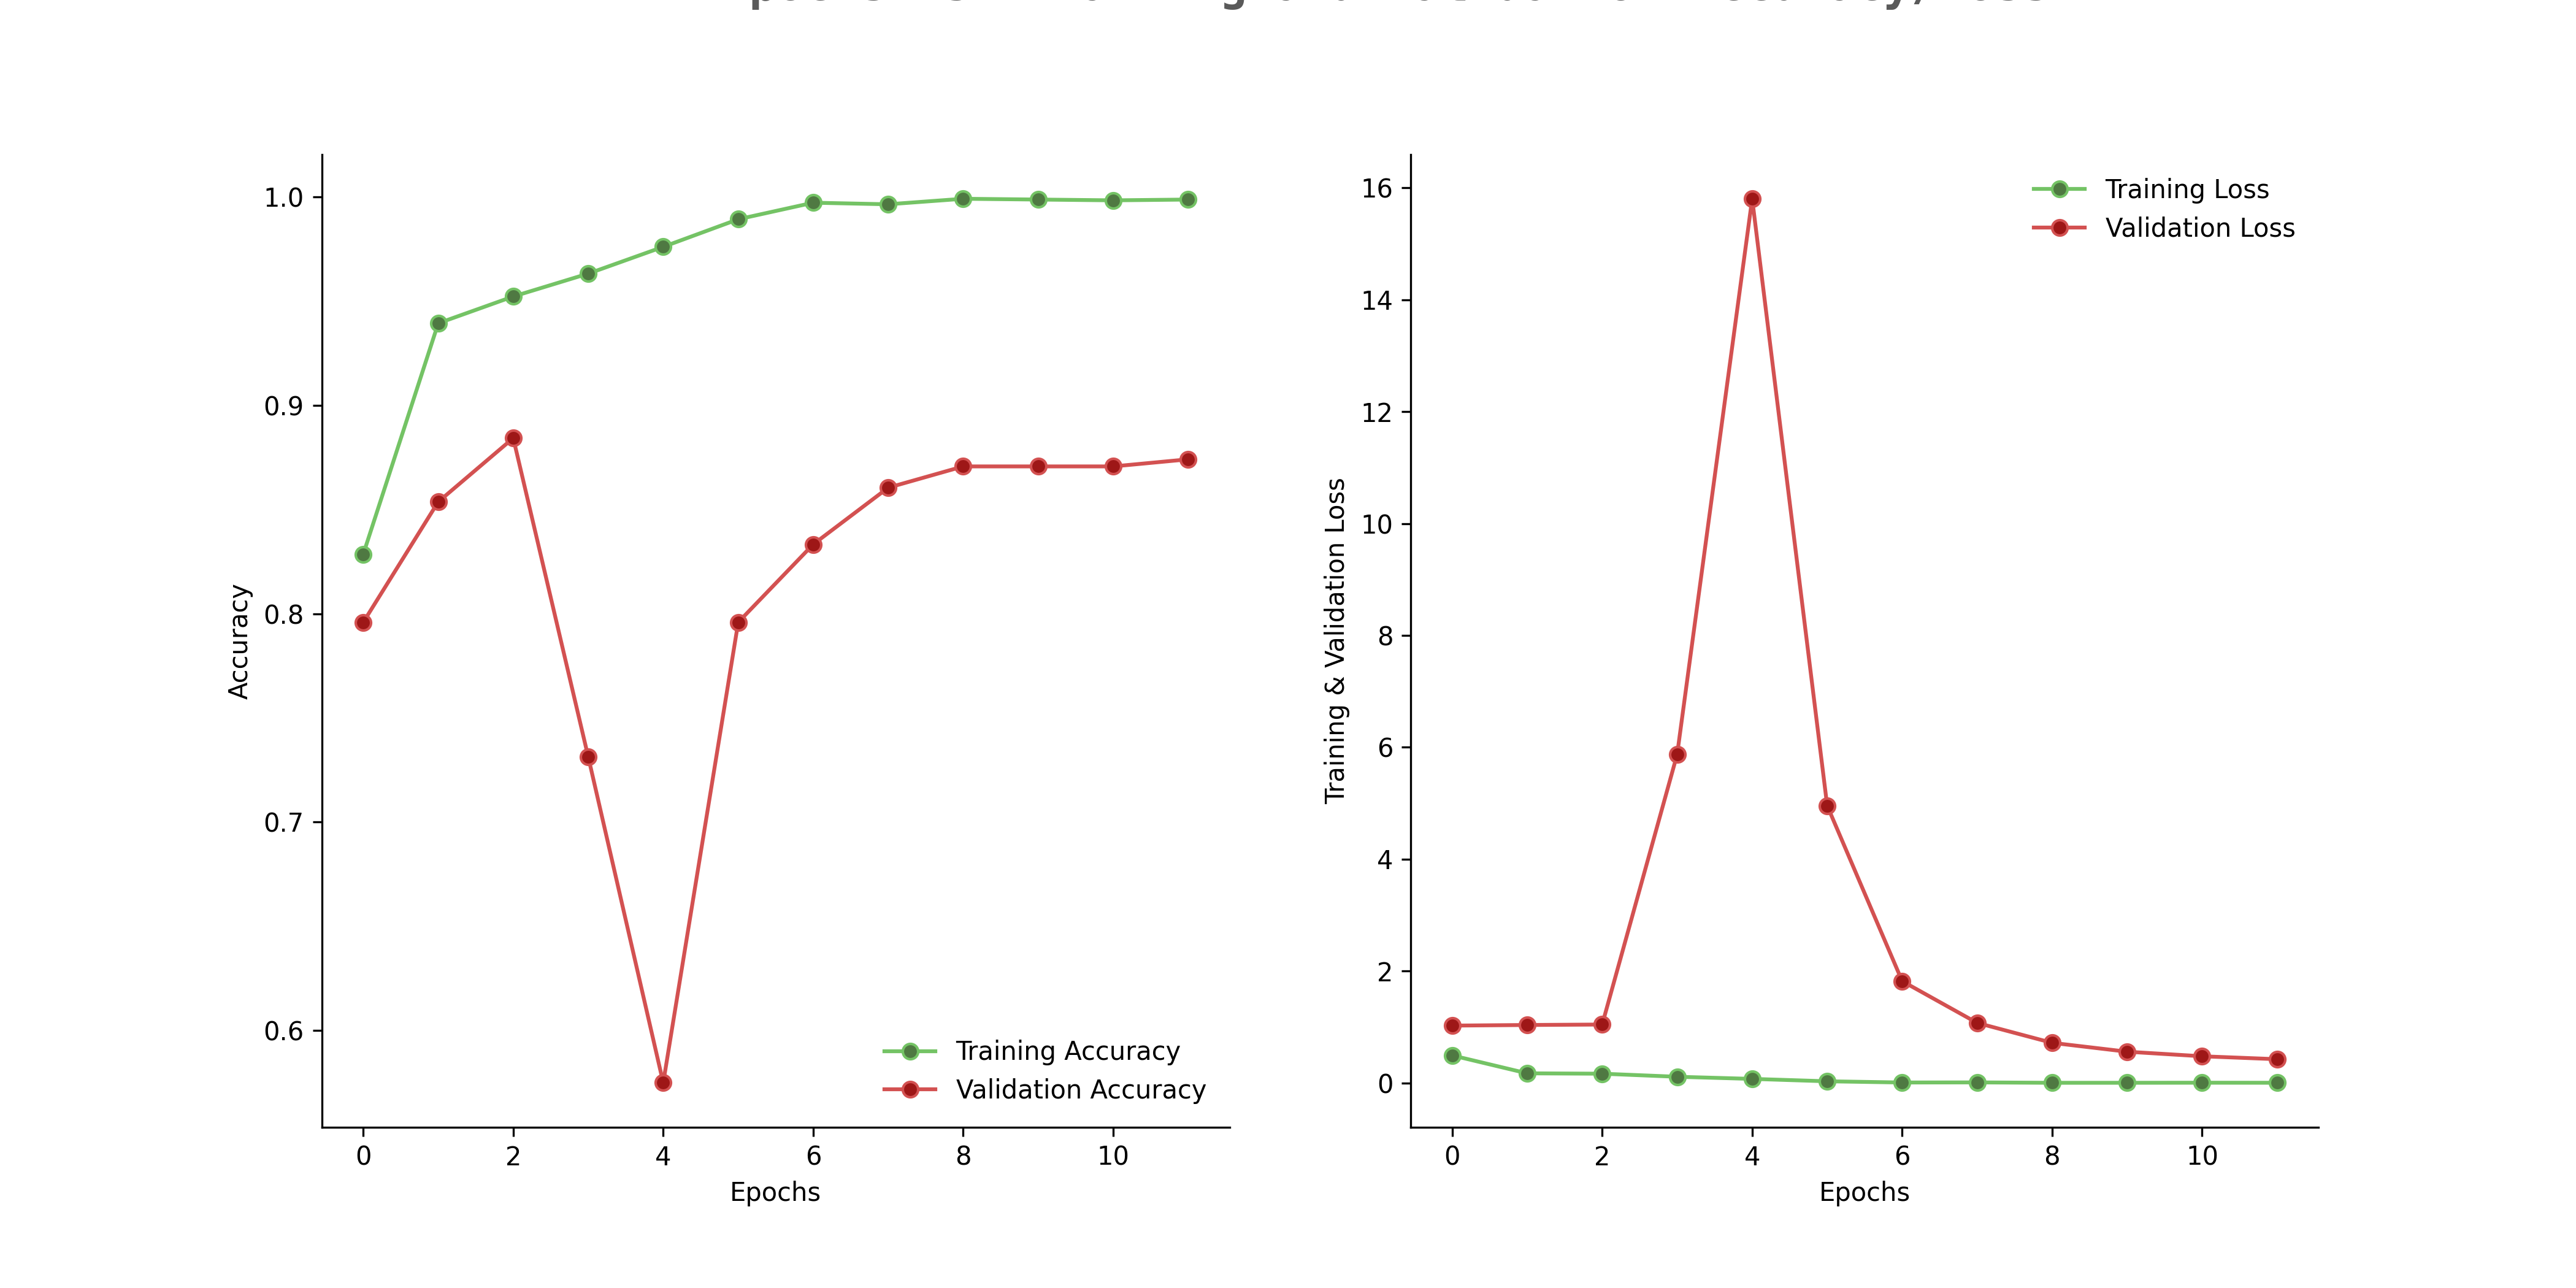
\includegraphics[scale=0.29]{Photos/MobileNetV3Large_plot.png}
\caption{Version 16 : MobileNetV3Large} \label{fig:mnetv3l}
\end{figure}
Figure \ref{fig:mnetv3s} shows the test loss vs epochs and test accuracy vs epoch graph of the model generated using MobileNetV3Small as the base model.
\begin{figure}[H]
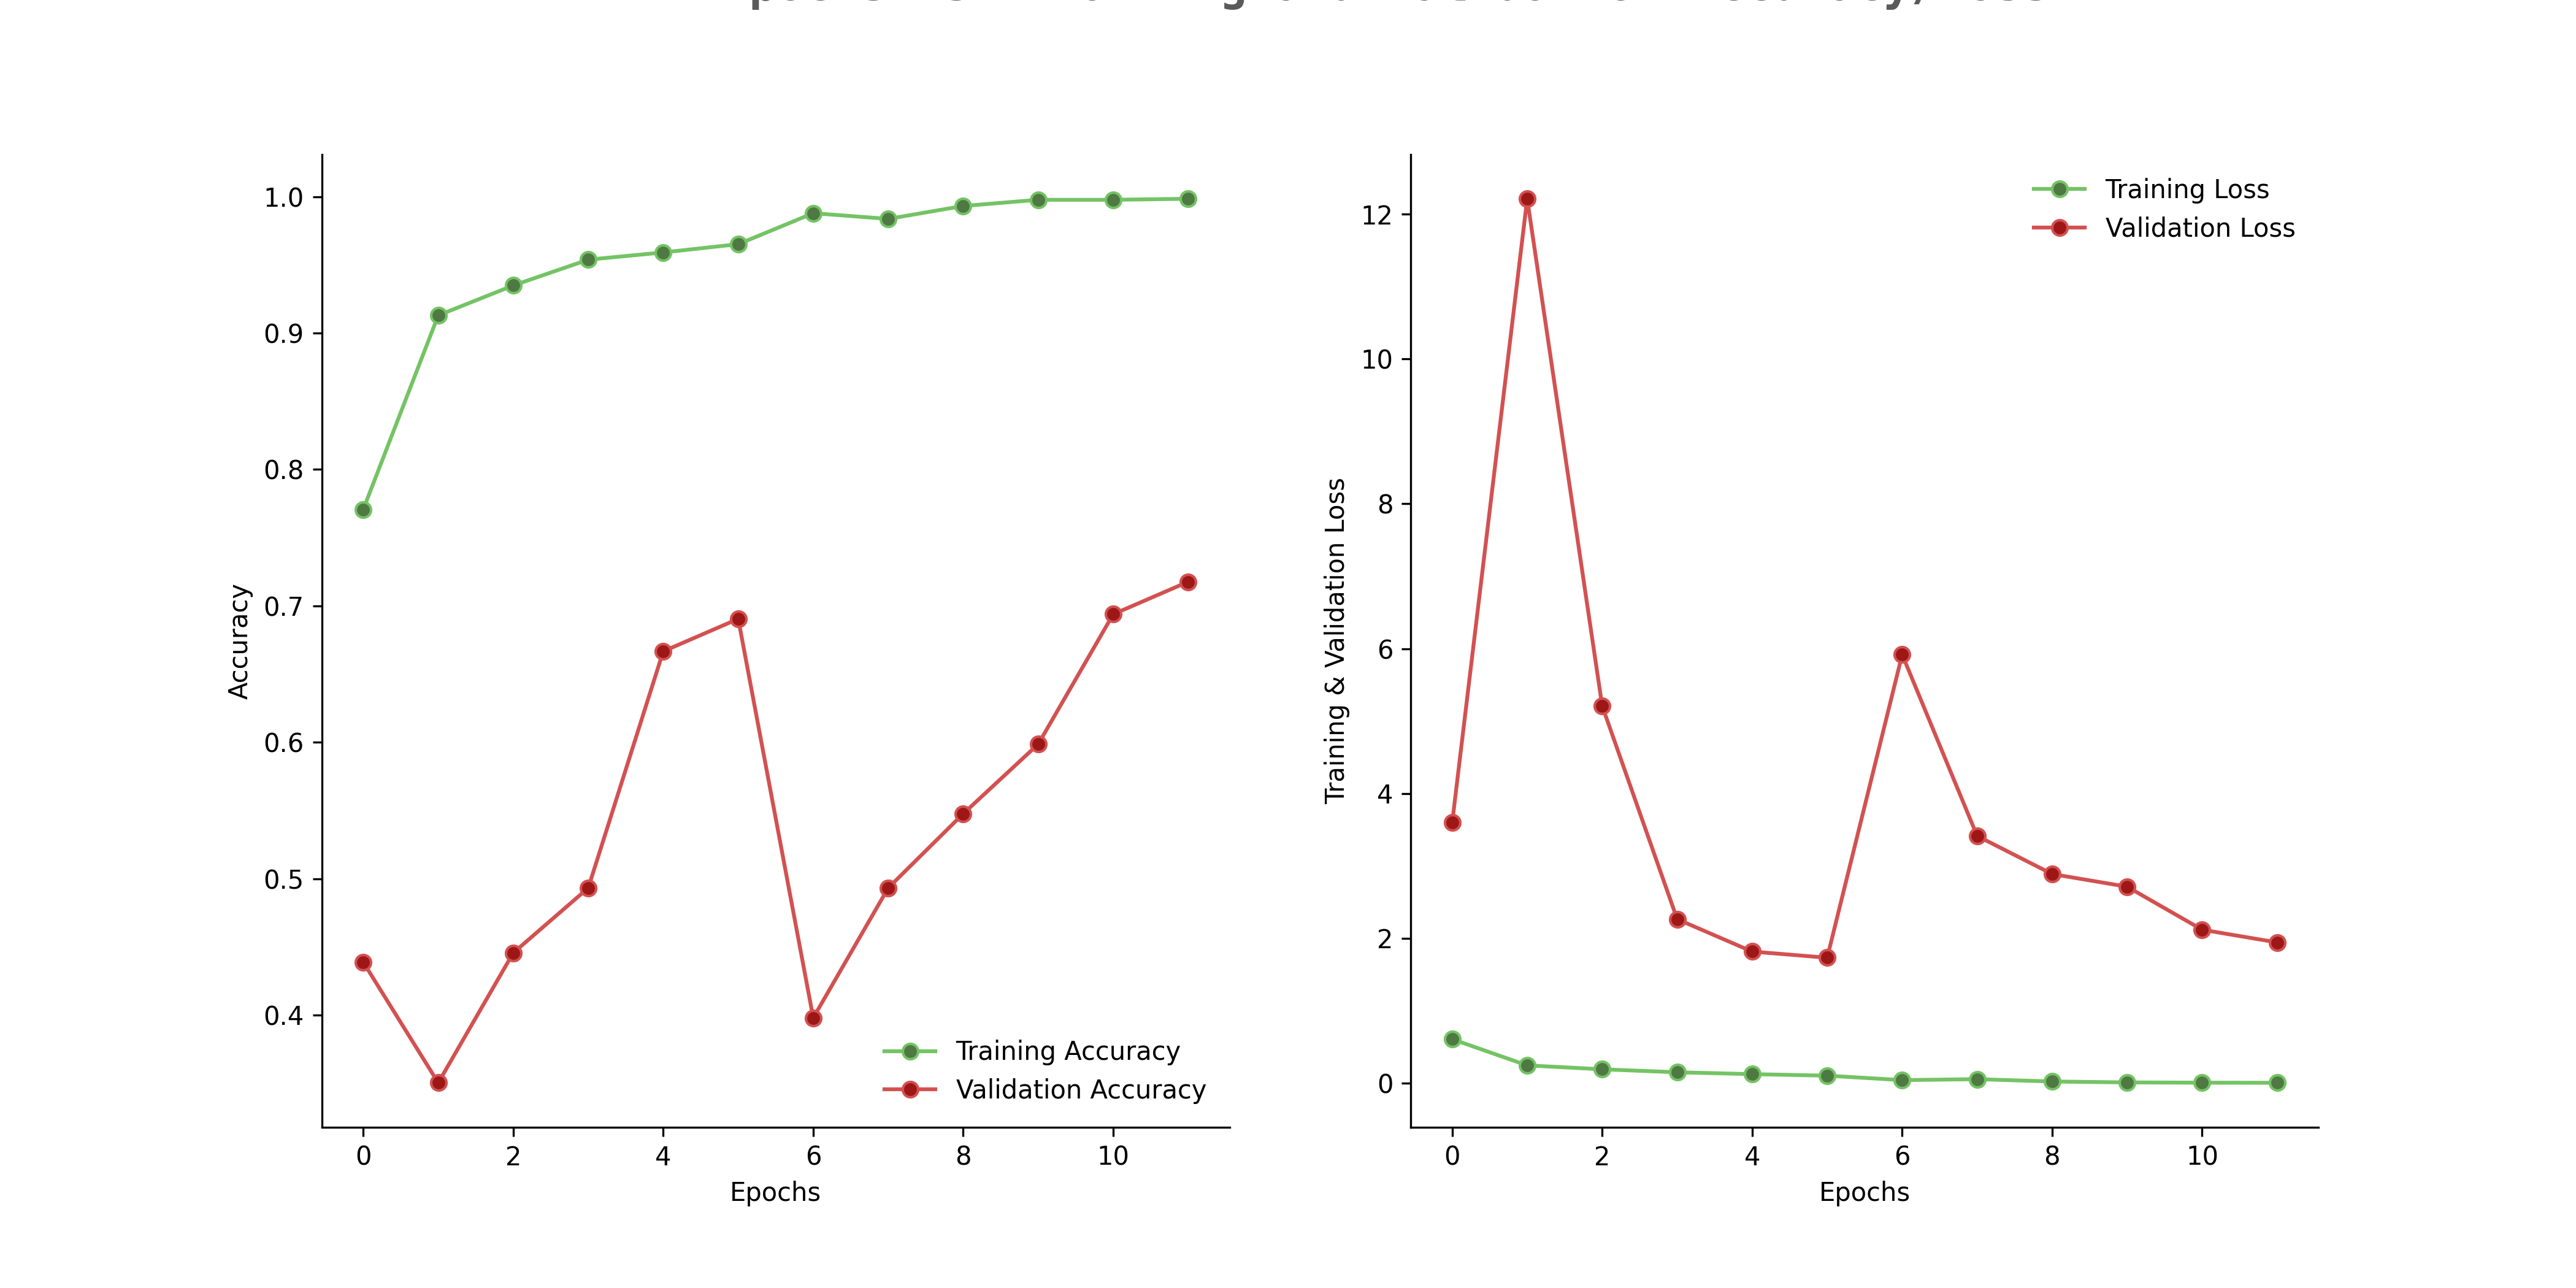
\includegraphics[scale=0.29]{Photos/MobileNetV3Small_plot.png}
\caption{Version 17 : MobileNetV3Small} \label{fig:mnetv3s}
\end{figure}
Figure \ref{fig:resnet101} shows the test loss vs epochs and test accuracy vs epoch graph of the model generated using ResNet101 as the base model.
\begin{figure}[H]
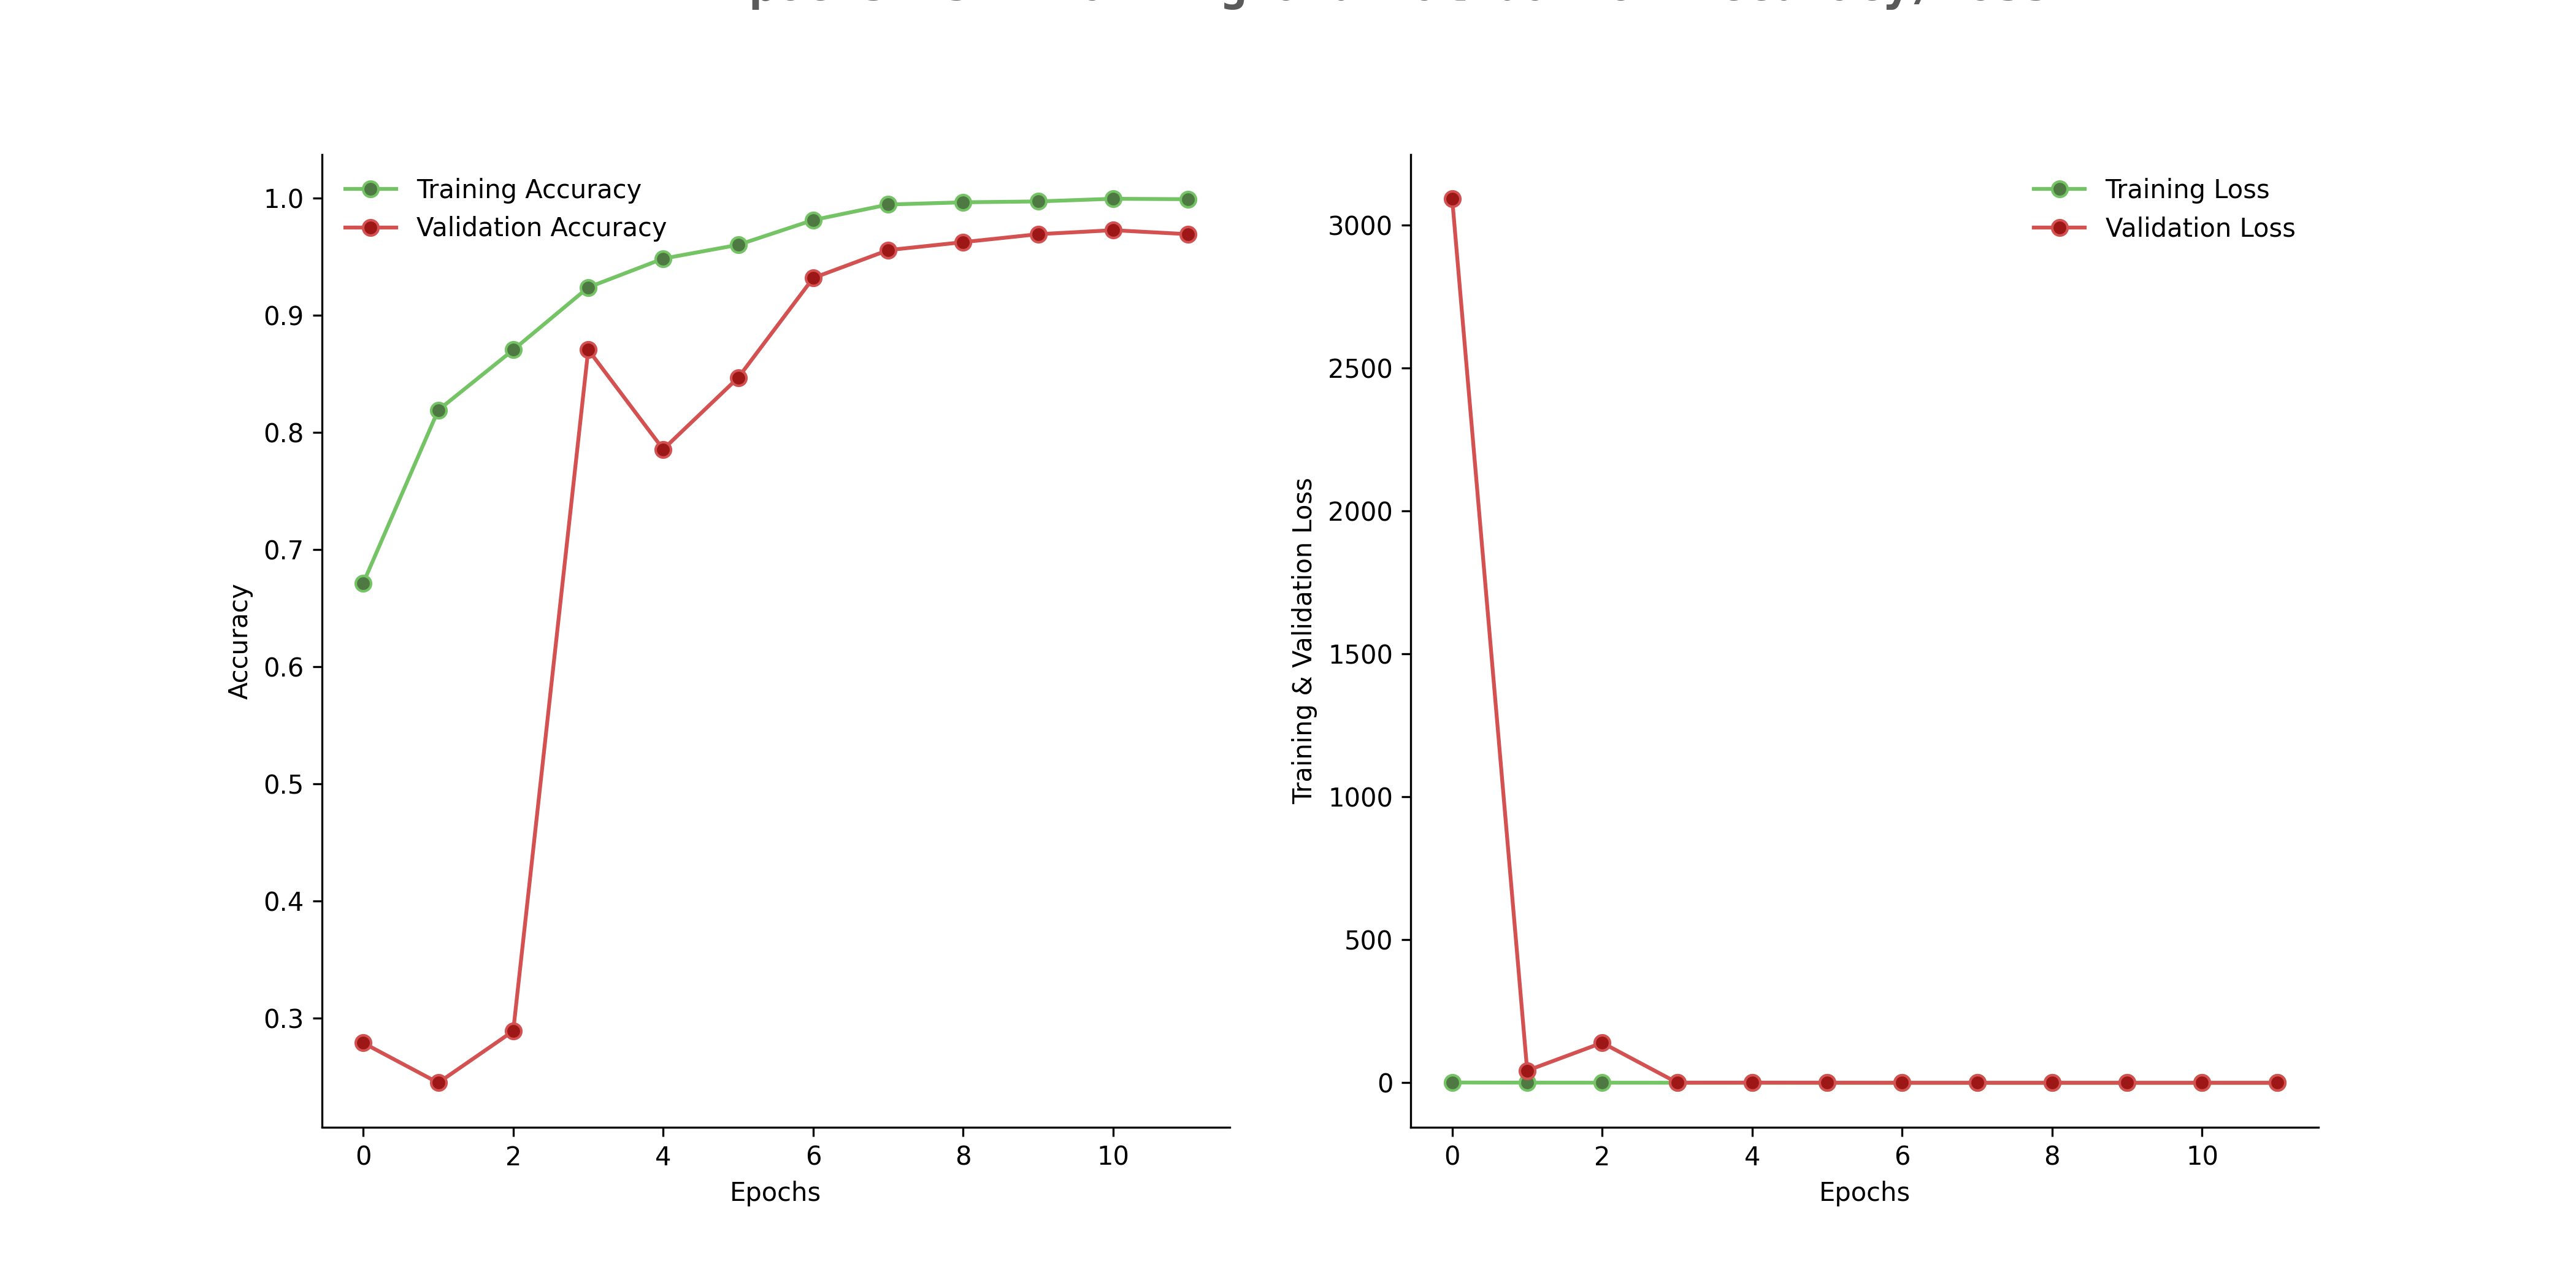
\includegraphics[scale=0.29]{Photos/ResNet101_plot.png}
\caption{Version 18 : ResNet101} \label{fig:resnet101}
\end{figure}
Figure \ref{fig:resnet101v2} shows the test loss vs epochs and test accuracy vs epoch graph of the model generated using ResNet101V2 as the base model.
\begin{figure}[H]
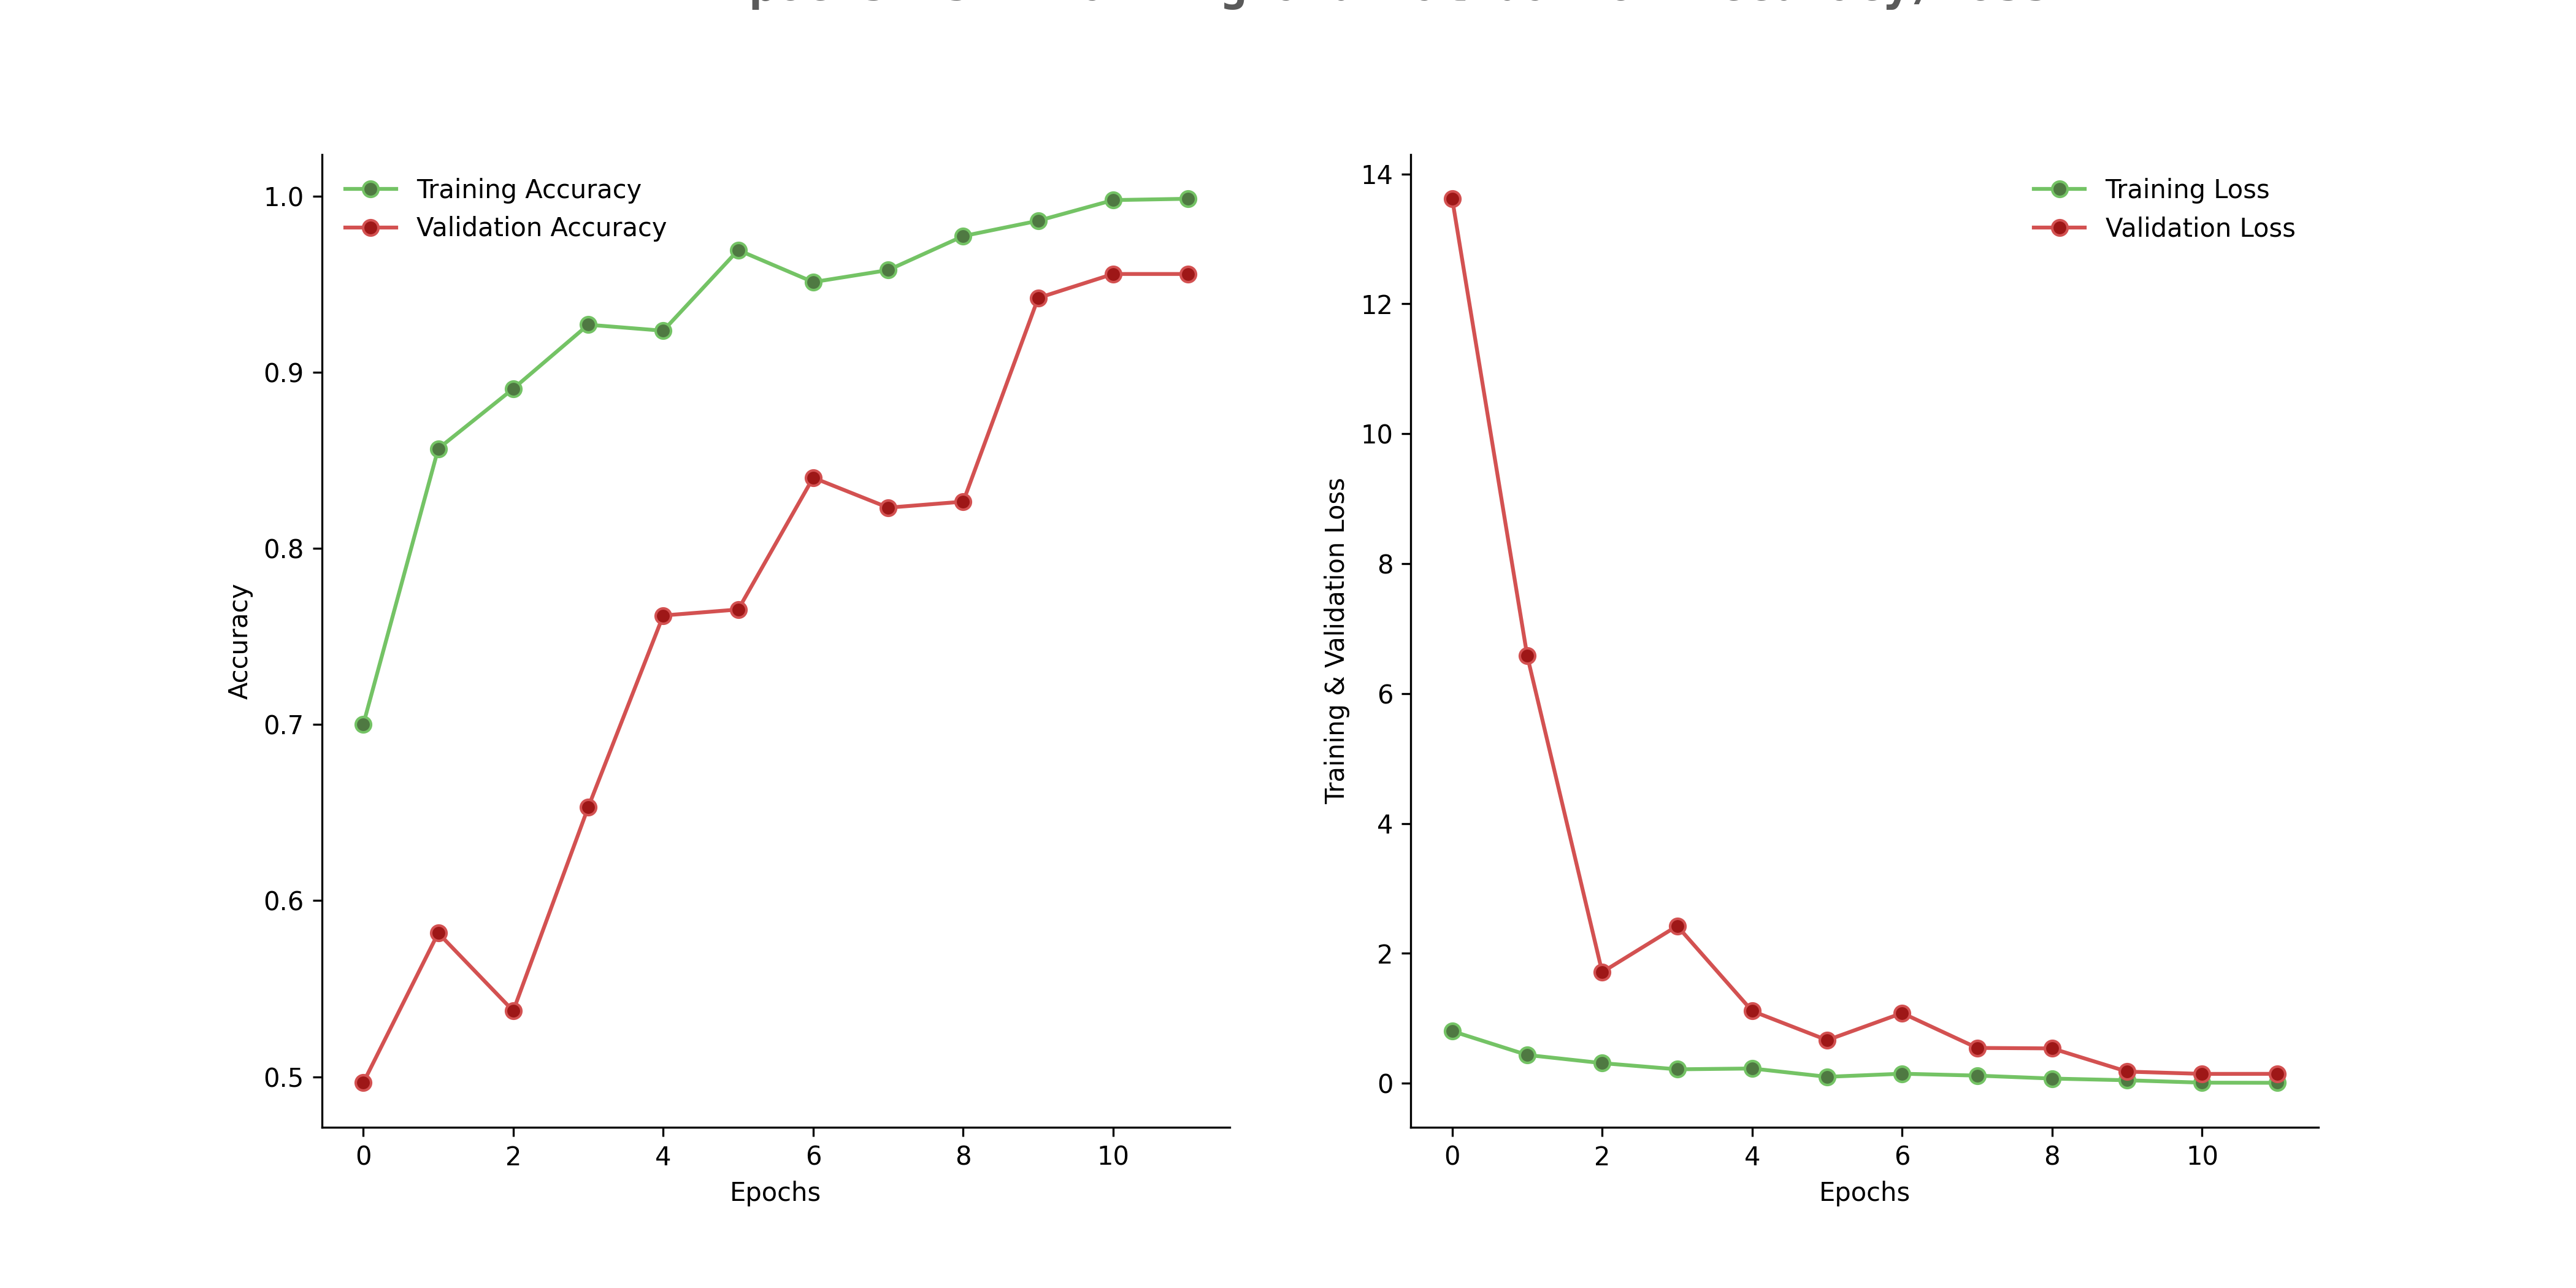
\includegraphics[scale=0.29]{Photos/ResNet101V2_plot.png}
\caption{Version 19 : ResNet101V2} \label{fig:resnet101v2}
\end{figure}

\section{Manual Test Results}
In Manual Testing images from an unbiased dataset is used to test the model on individual images. The images from the unbiased dataset have not been used to training of the model at any point; hence it acts as unbiased data. The results from the manual testing are as follows:
\begin{itemize}
    \item Glioma Tumour Present in the Brain:
        \begin{figure}[H]
        \frame{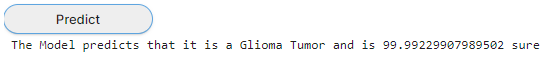
\includegraphics[scale=0.9]{Photos/Resule_glio_.PNG}}
        \caption{Glioma Tumour Manual Testing Results} \label{fig:glioma_res}
        \end{figure}
    \item Meningioma Tumour Present in the Brain:
        \begin{figure}[H]
        \frame{
\includegraphics[scale=0.9]{Photos/Resule_meni_.png}}
        \caption{Meningioma Tumour Manual Testing Results} \label{fig:menin_res}
        \end{figure}
    \item Pituitary Tumour Present in the Brain:  
        \begin{figure}[H]
        \frame{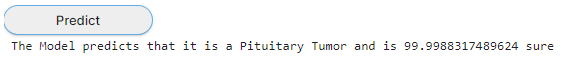
\includegraphics[scale=0.9]{Photos/Resule_pitu_.PNG}}
        \caption{Pituitary Tumour Manual Testing Results} \label{fig:pitu_res}
        \end{figure}
    \item Tumour Absent in the Brain:  
        \begin{figure}[H]
        \frame{
\includegraphics[scale=0.9]{Photos/Resule_no_.PNG}}
        \caption{No Tumour Manual Testing Results} \label{fig:no_tumour_res}
        \end{figure}   
\end{itemize}

\section{Terminal logs for starting the Web Application}
The figure \ref{fig:initial_commit} displays the initial commit which is used for, starting the web application. We use the command "streamlit run filename.fileextention" to start the streamlit server. The figure \ref{fig:terminal_log} displays the terminal logs post server deployment. Once the "streamlit run filename.fileextension" command has been executed, the server begins running and provides with a local server link for deploying it to the local browser. This local server link is as follows: "Local URL: http://localhost:8501" and "Network URL: http://172.27.112.252:8501". This log also will contain every backend process that occurs within the web application, like uploading an image, or processing some data.
\begin{figure}[H]
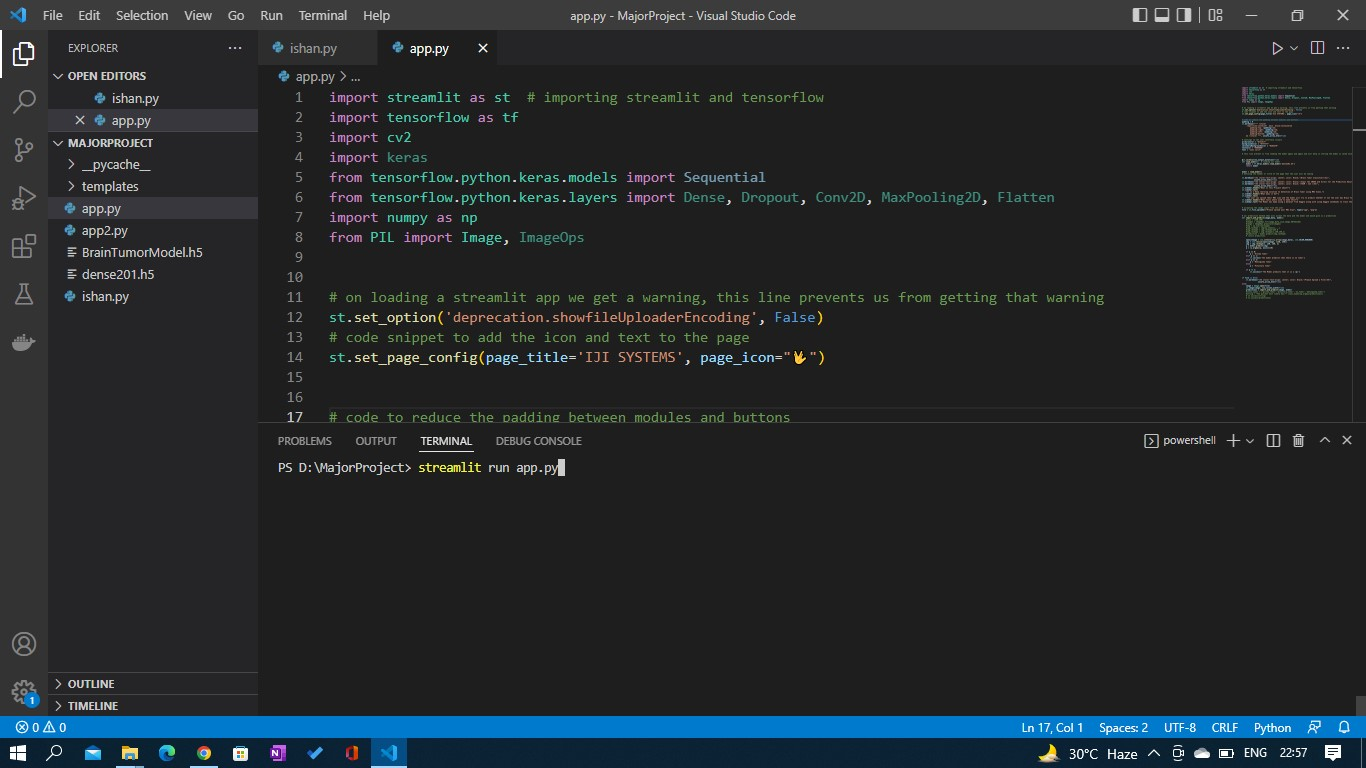
\includegraphics[scale=0.38]{Photos/Initial_command_terminal.jpg}
\caption{Initial Terminal Commit} \label{fig:initial_commit}
\end{figure}
\begin{figure}[H]
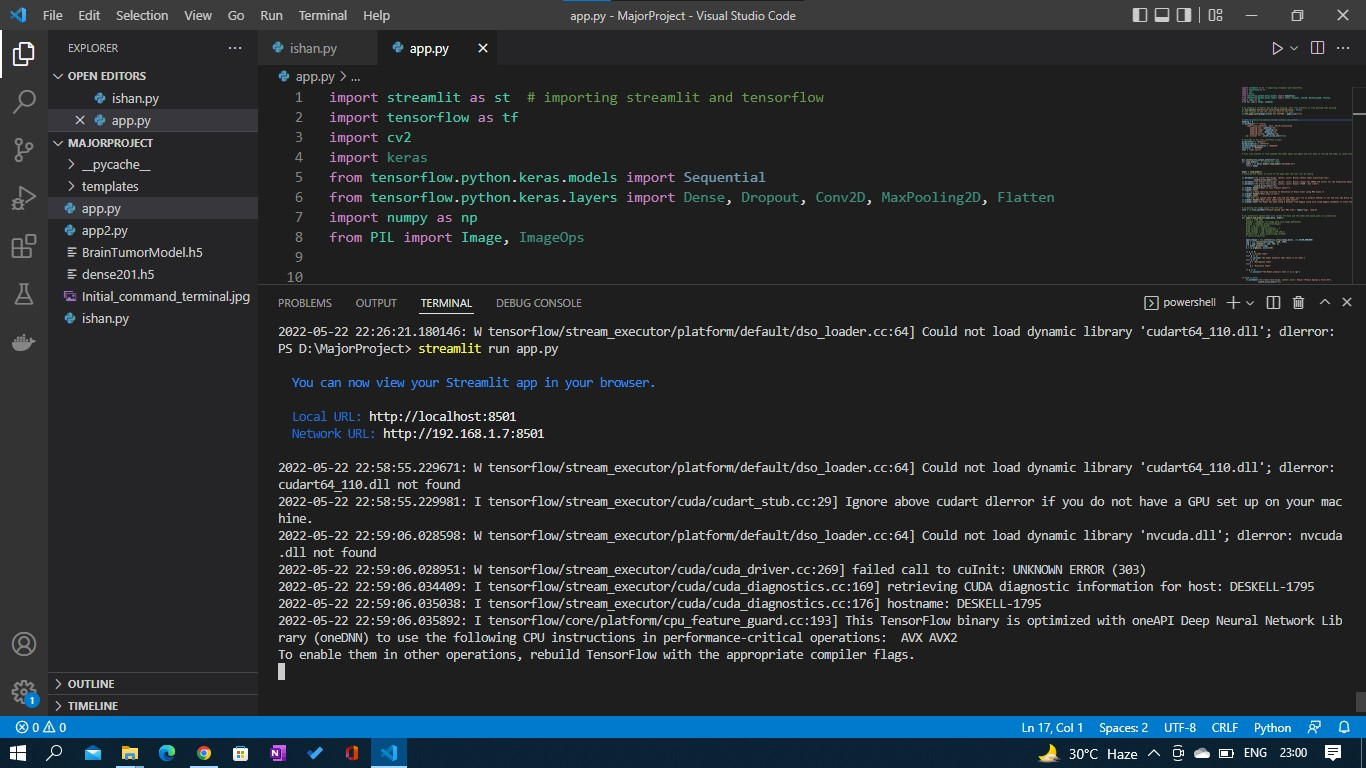
\includegraphics[scale=0.38]{Photos/Terminal_Logs_appStarts.jpg}
\caption{Terminal Logs when Application starts} \label{fig:terminal_log}
\end{figure}

\section{Web Application User Interface}
The web application has been developed using Streamlit framework. Figure \ref{fig:UI_sidebar} shows the comprehensive web application front end constituents where it has a sidebar on the left side and central area of the web app has the welcome page. This sidebar contains the navigation of the application, thereby enabling to change to different routes based on the user choice.

\begin{figure}[H]
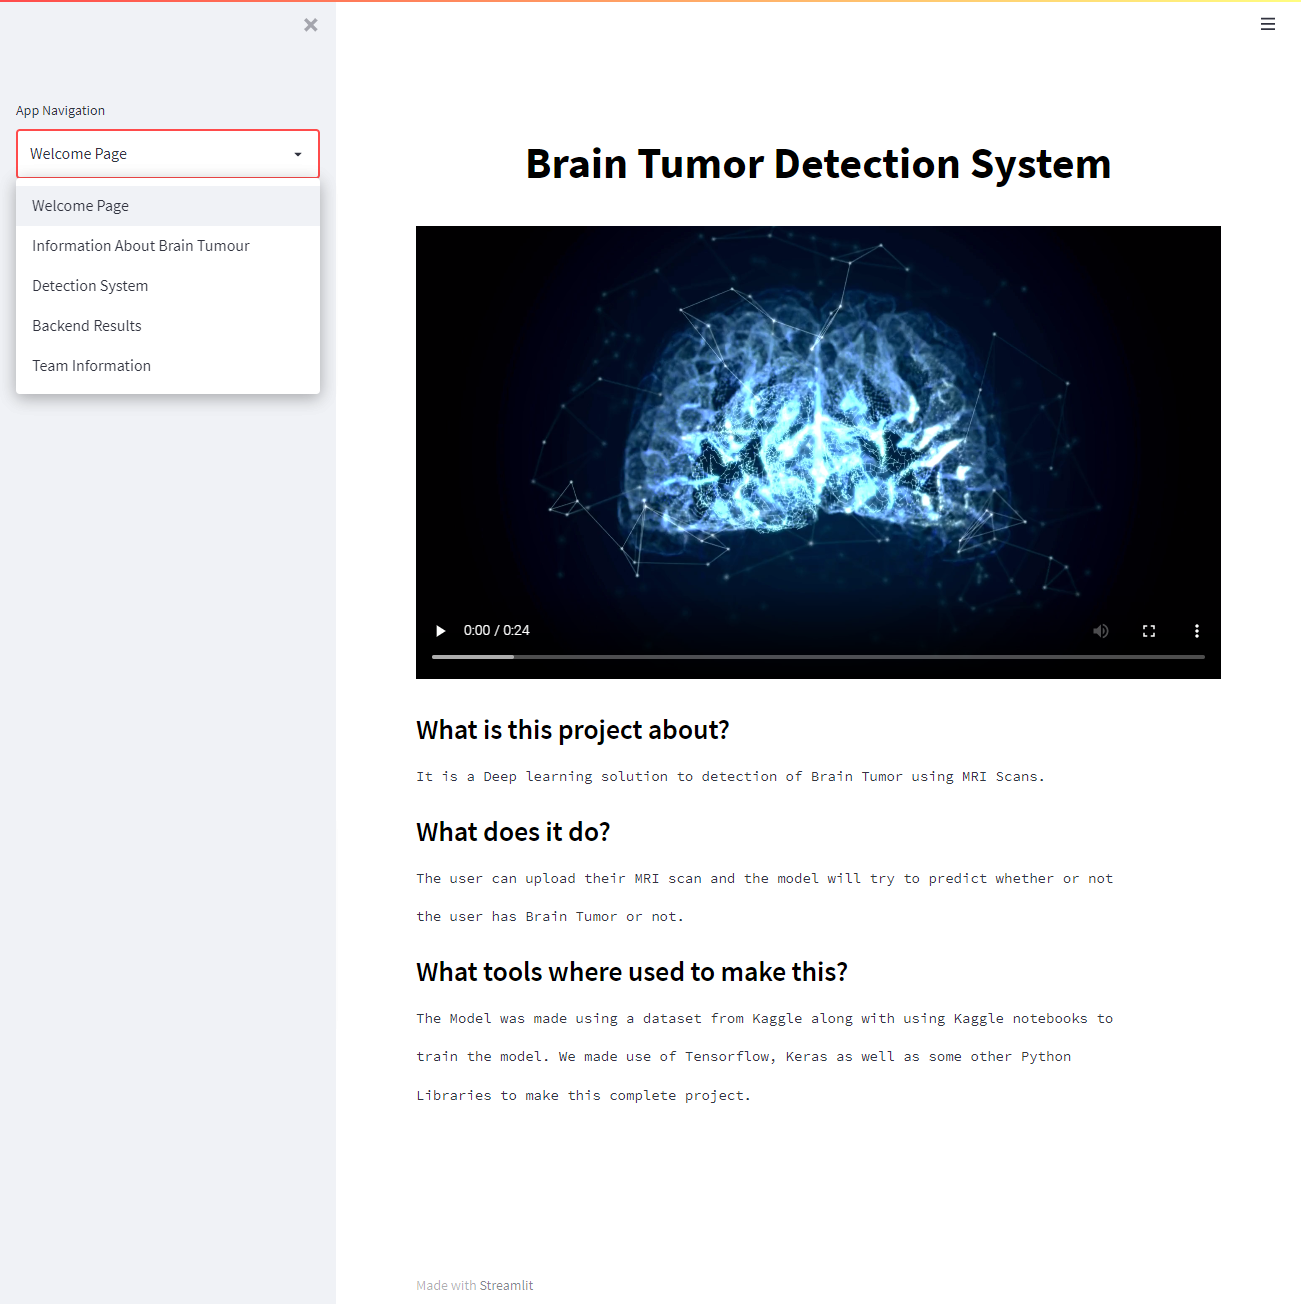
\includegraphics[scale=0.3]{Photos/UI_with_sidebar.png}
\caption{User Interface with sidebar} \label{fig:UI_sidebar}
\end{figure}

Figure \ref{fig:page1} is the first page or route of the web application which is having the welcome page and information about how this model works with a video animation embedded on top. The route also highlights the tools used to make the application.
\begin{figure}[H]
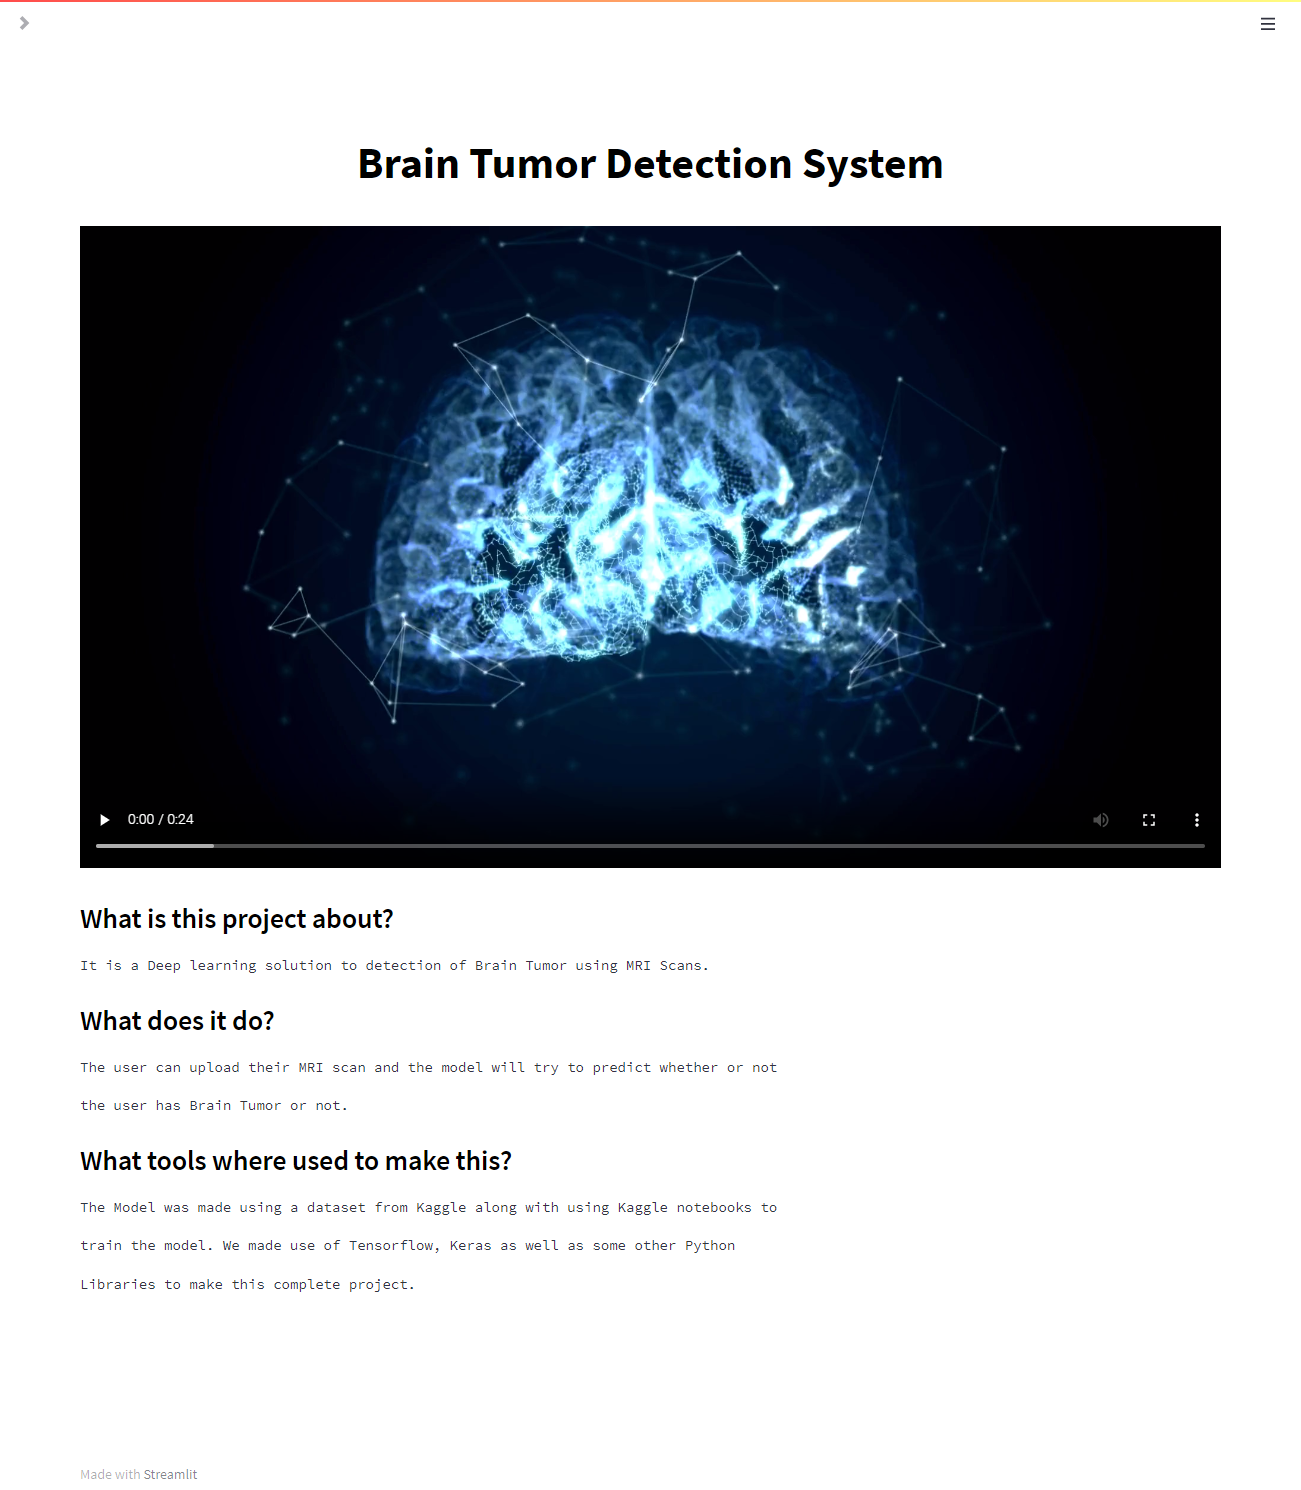
\includegraphics[scale=0.3]{Photos/Page1.png}
\caption{Welcome Page} \label{fig:page1}
\end{figure}

Figure \ref{fig:page2} is the information page route of the web application which has interactivity with the information mentioned about brain tumours, it's types, diagnosis, awareness and the treatment methods. It has the hyperlinks connected for displaying more information about the particular type of tumour and treatment methods. The page gives a brief insight into three types of tumors in particular : glioma tumor, pituitary tumor, and meningioma tumor.
\begin{figure}[H]
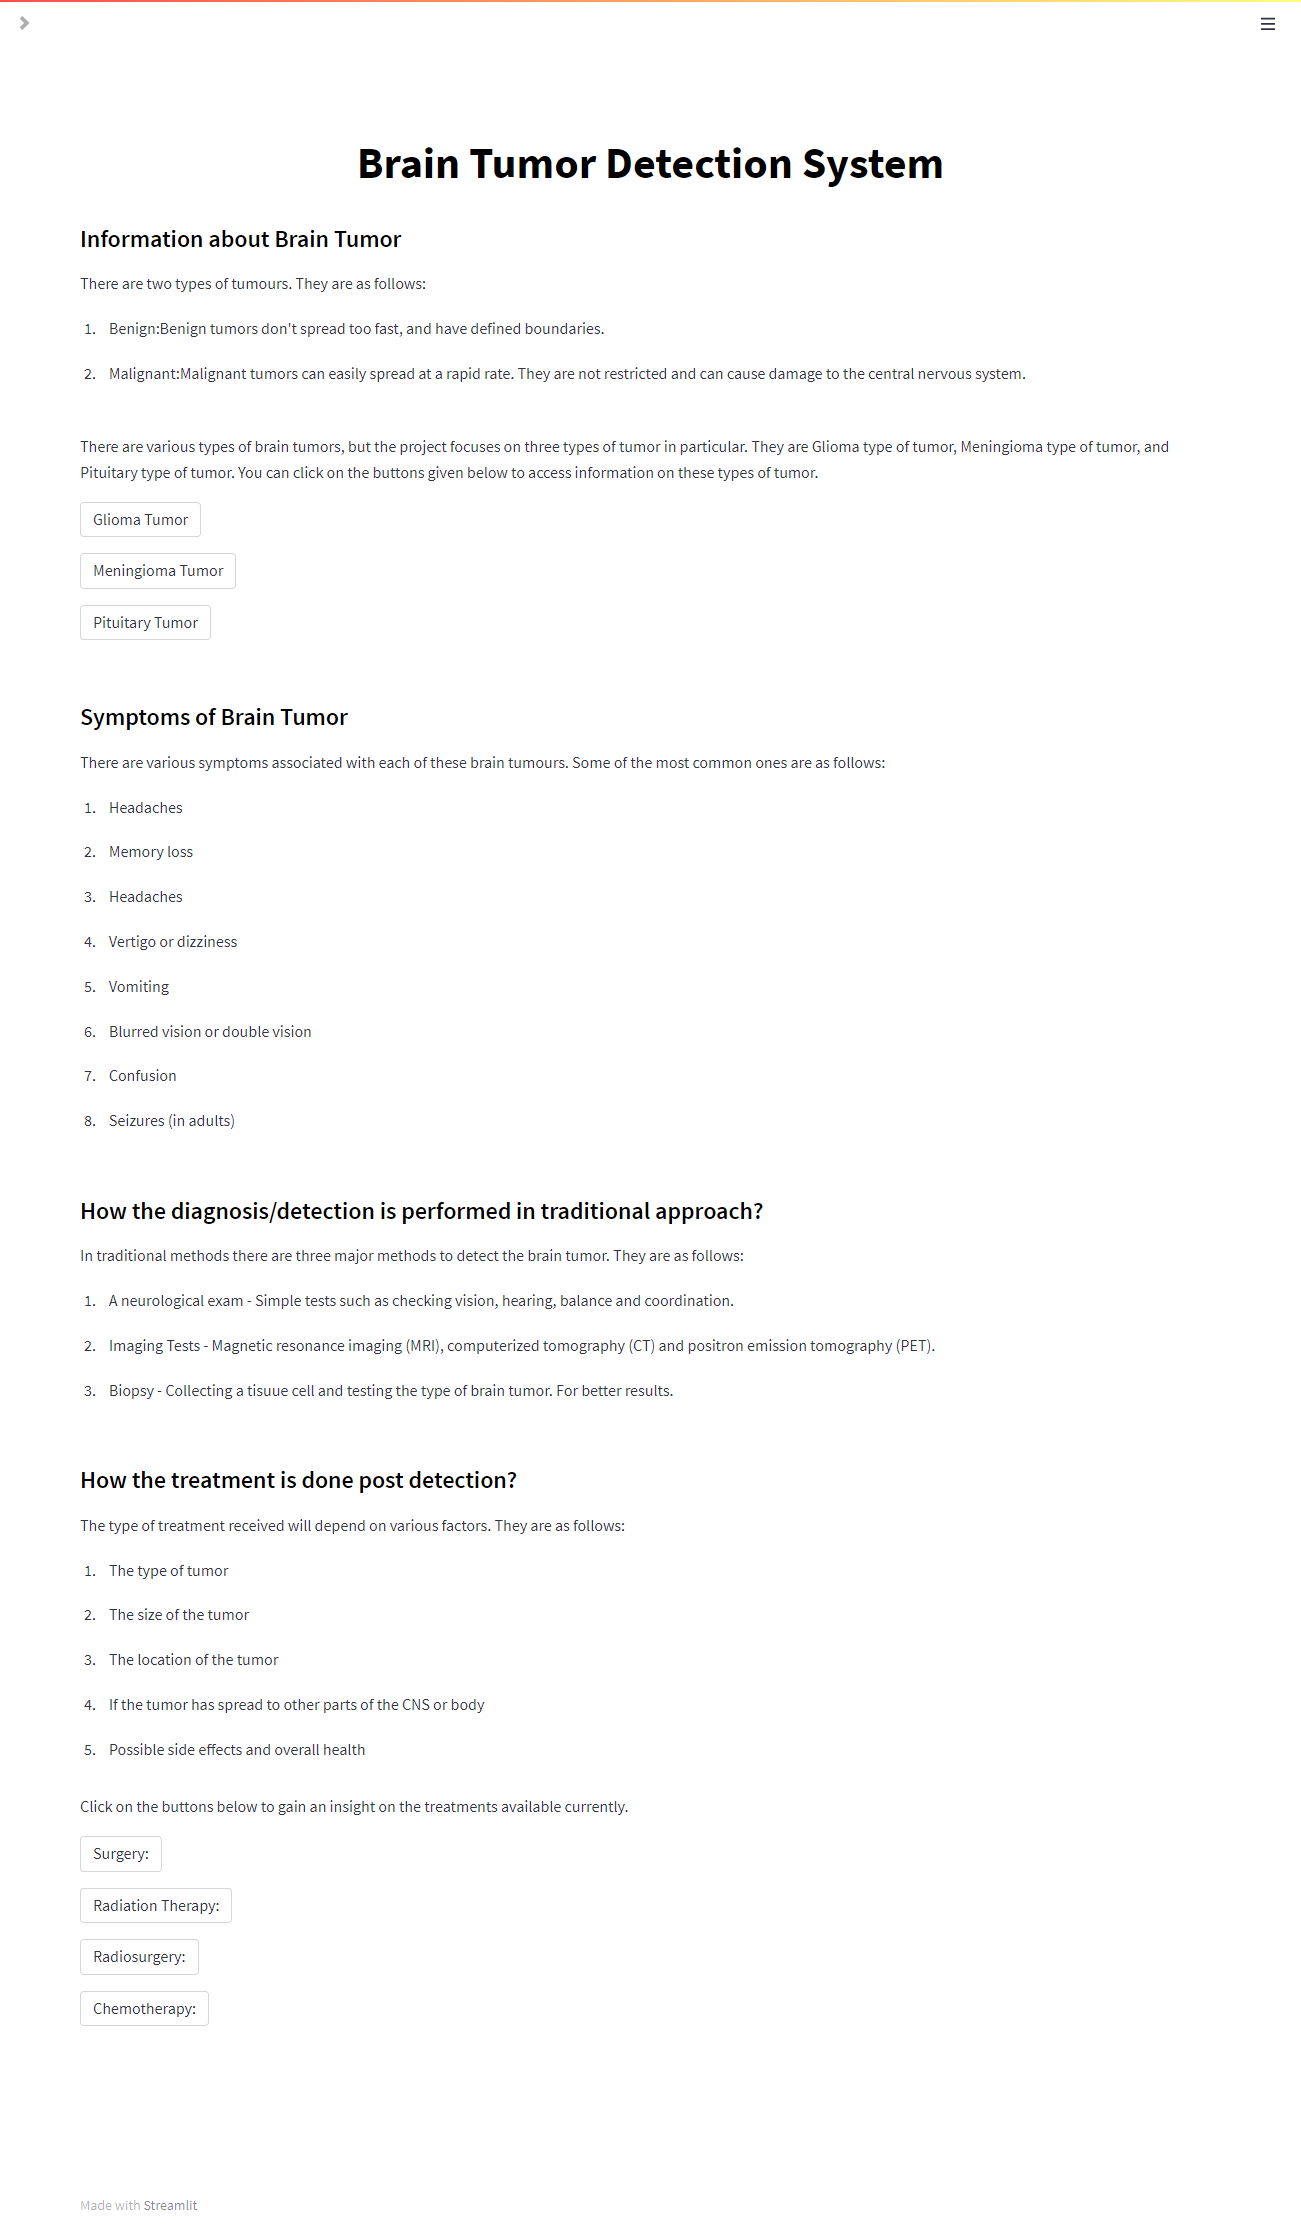
\includegraphics[scale=0.3]{Photos/Page2.png}
\caption{Brain Tumor Information Page} \label{fig:page2}
\end{figure}

Figure \ref{fig:page3} is the main detection model system which has the constituents of a input dialog box with specified memory size and format of the image which acts as input to the detection model. After model detects , it shows what type of tumour it is and a small description about the tumour found on the image. The web application also prints a confidence score as to how much the model has confidence that the particular uploaded image is of that type of label. 
\begin{figure}[H]
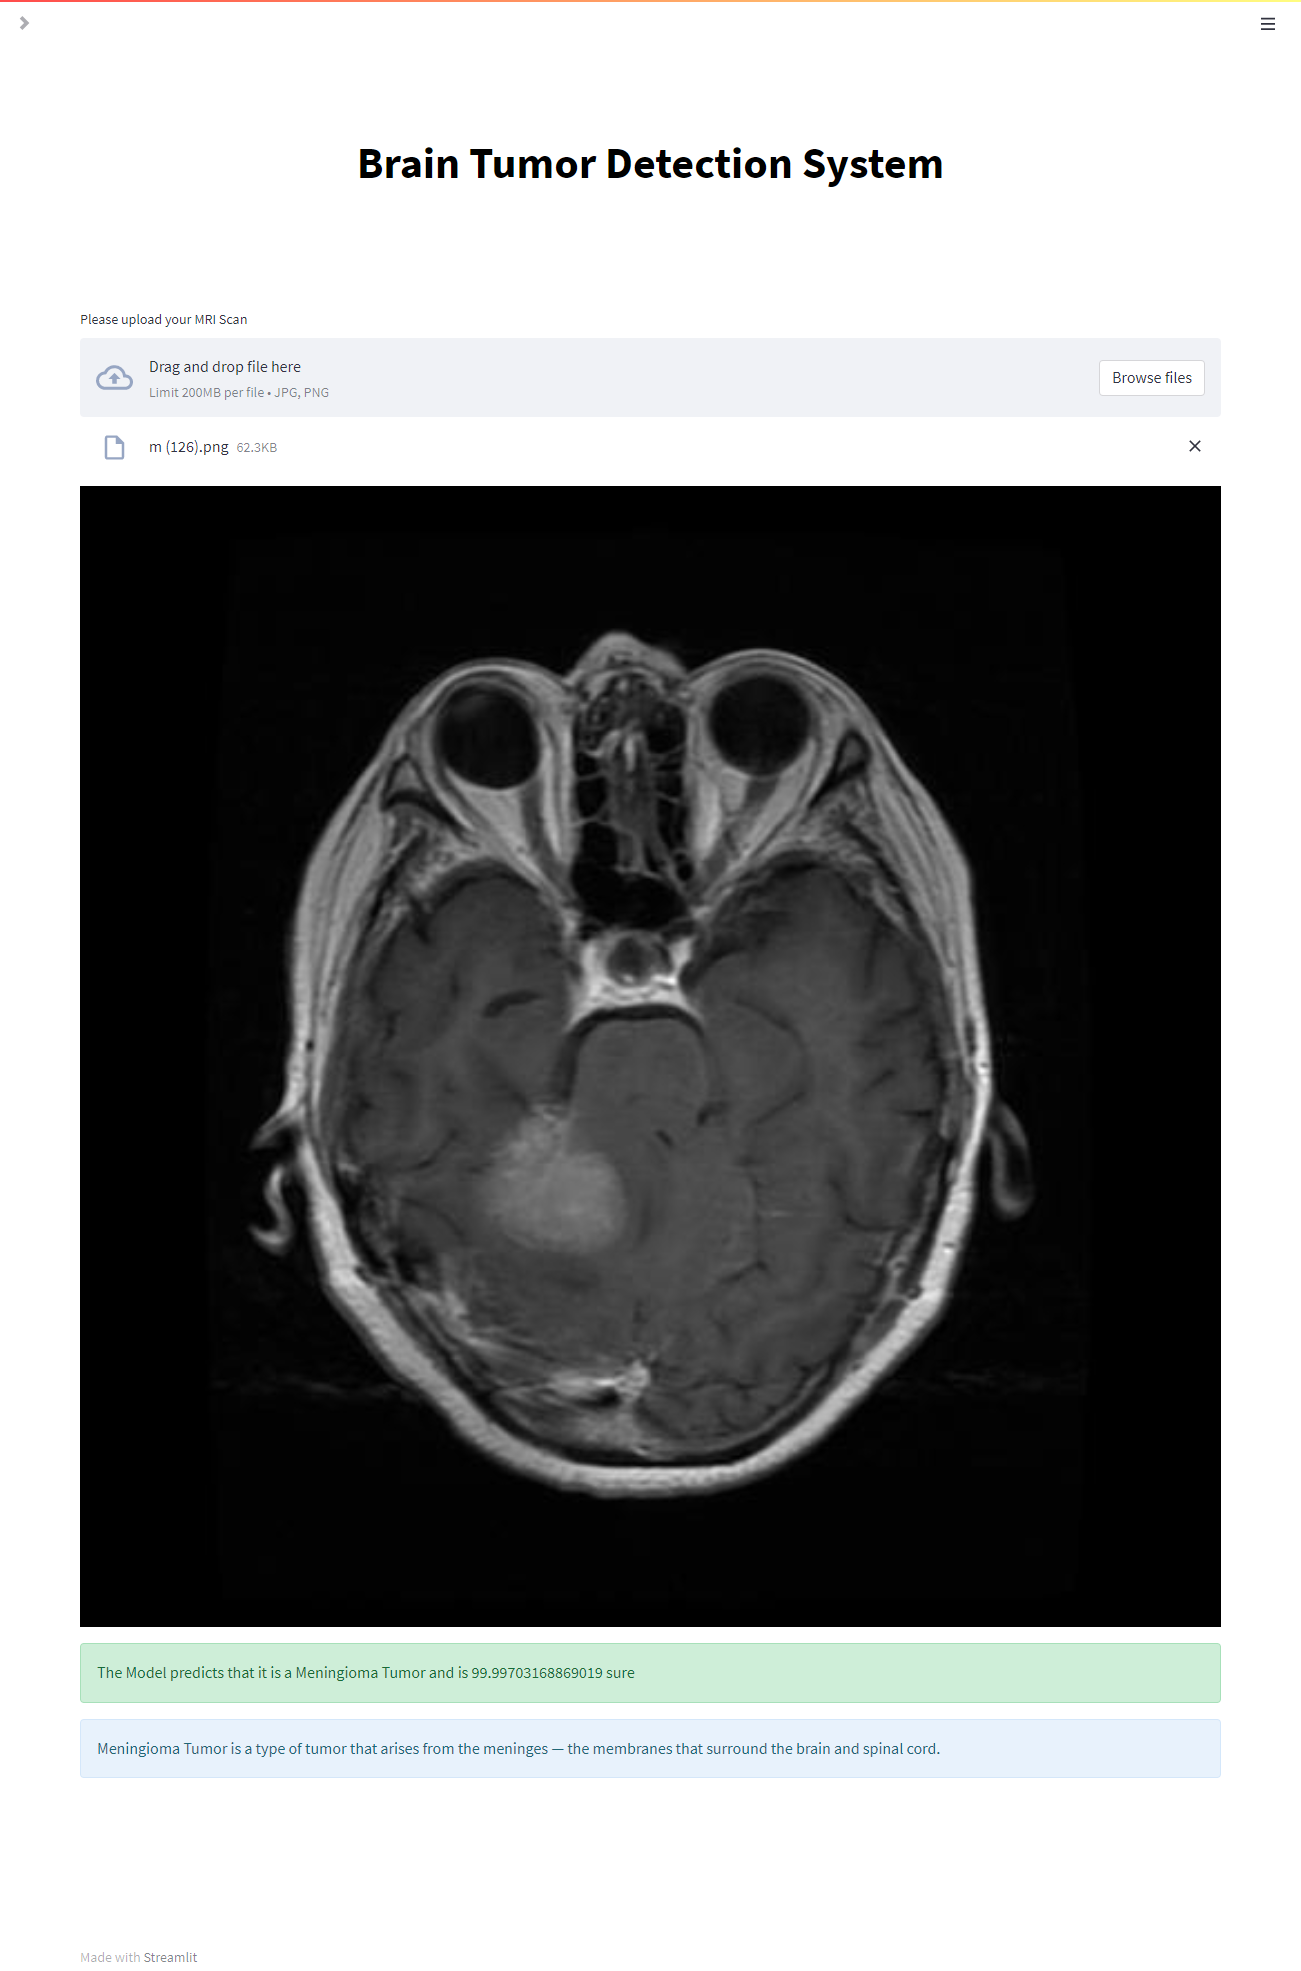
\includegraphics[scale=0.22]{Photos/Resule_meni_web.png}
\caption{Detection Page} \label{fig:page3}
\end{figure}

Figure \ref{fig:page4} shows the general backend result images which includes classification report, confusion matrix and explanation. 
\begin{figure}[H]
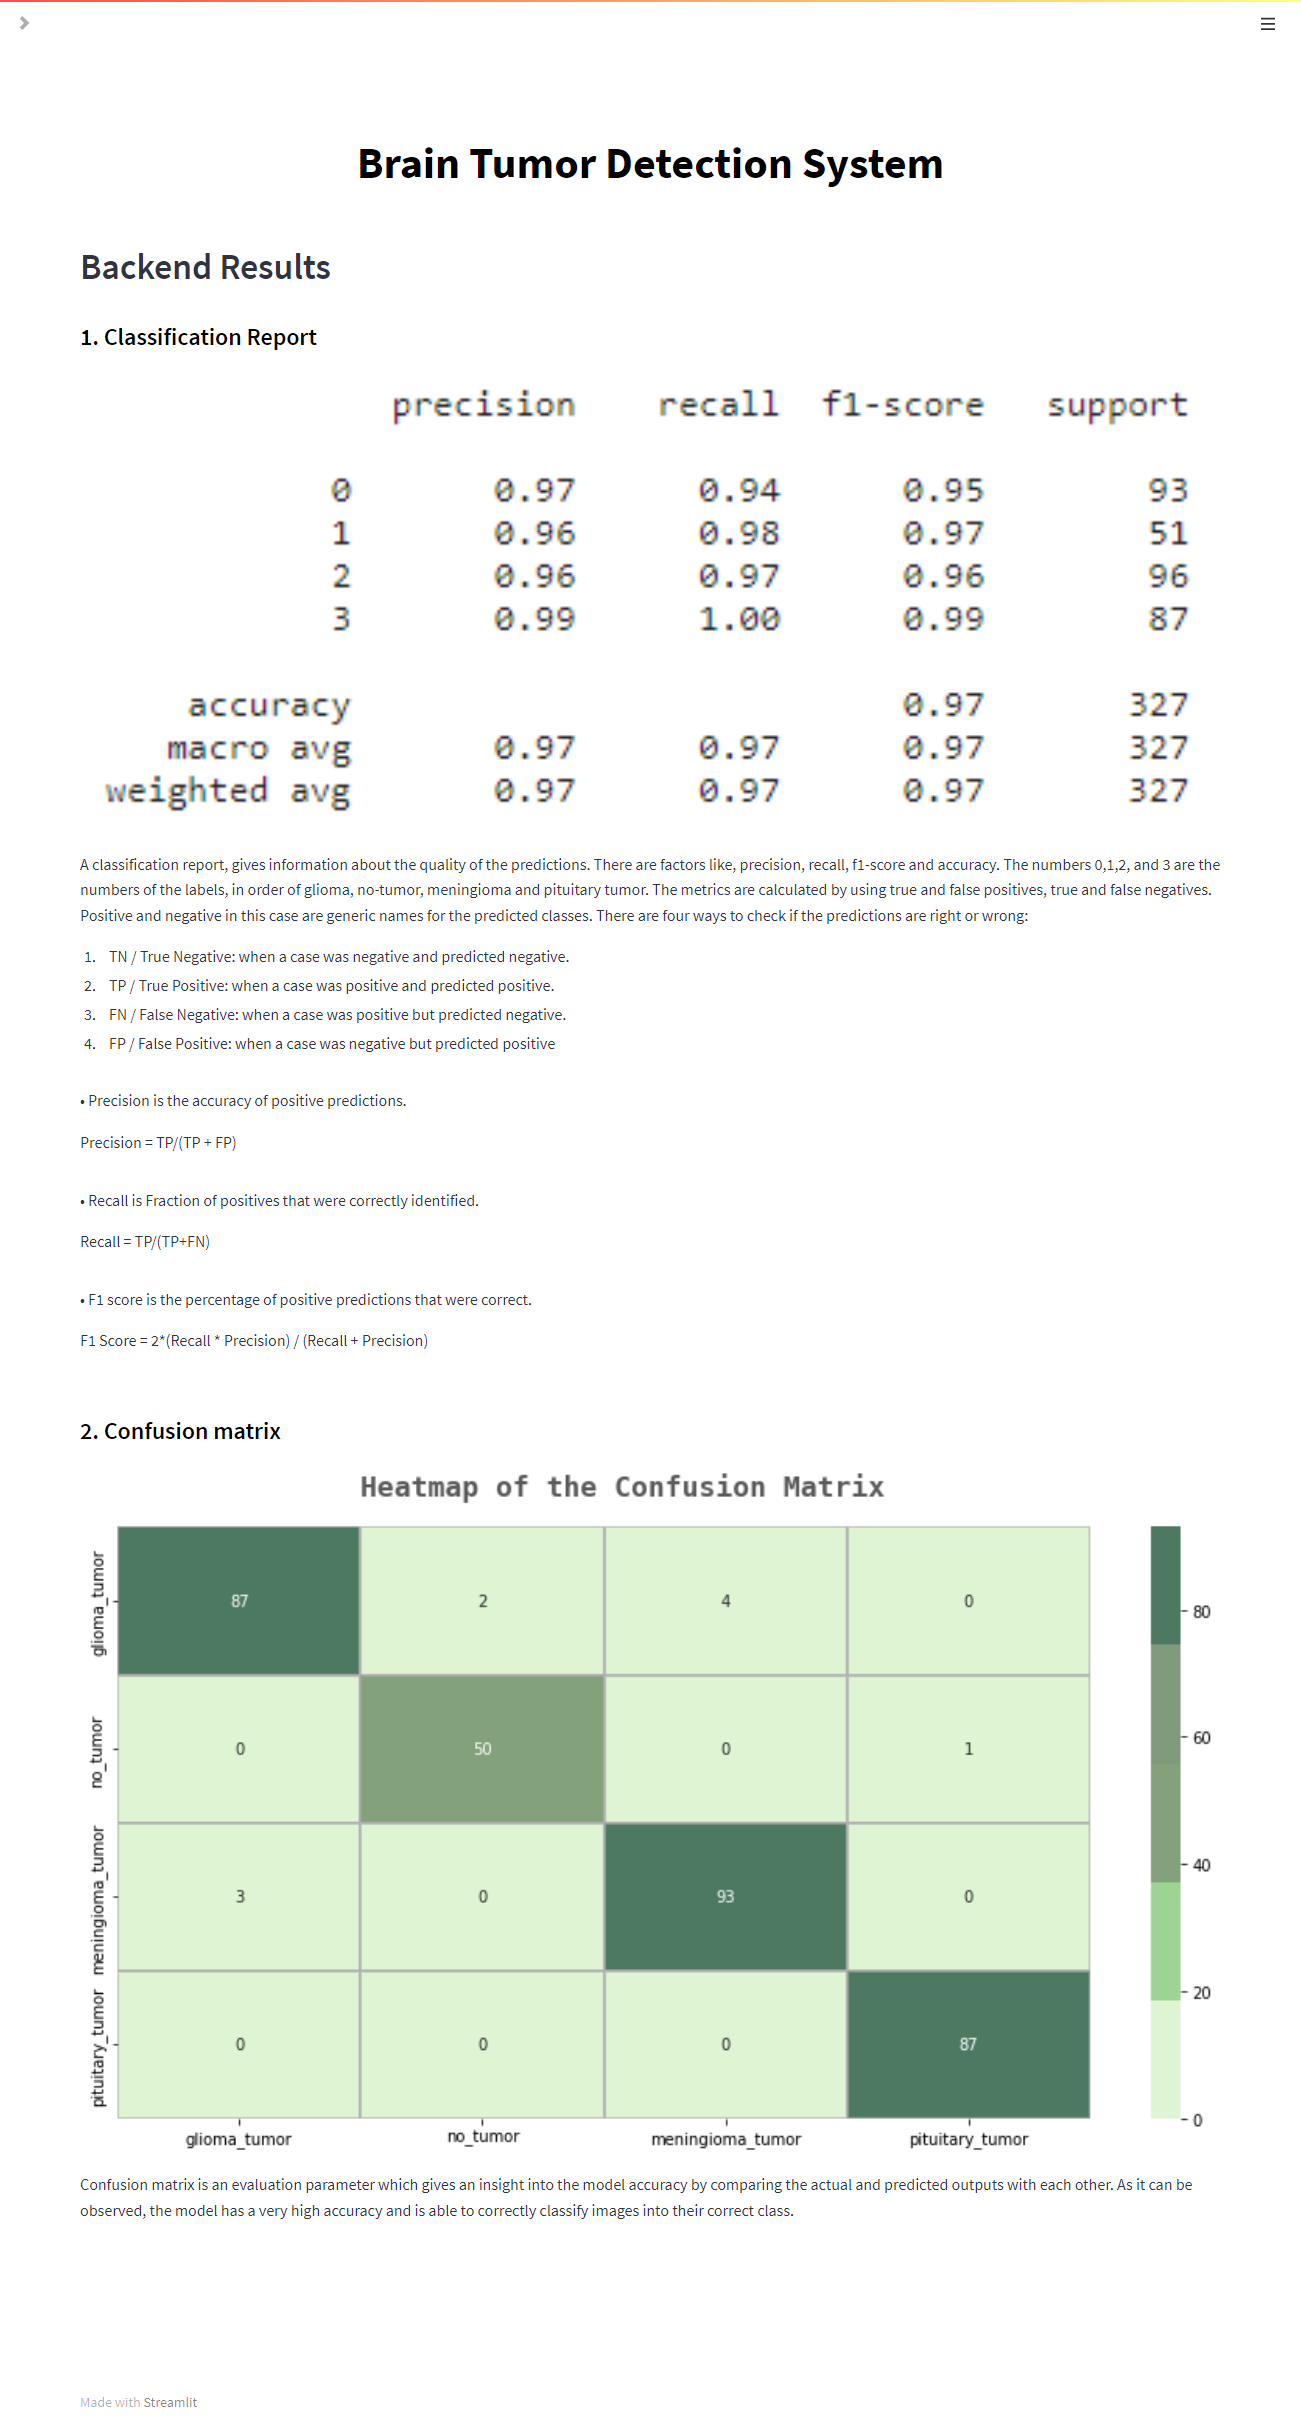
\includegraphics[scale=0.28]{Photos/Page4.png}
\caption{Backend Results} \label{fig:page4}
\end{figure}

Figure \ref{fig:page5} is the route screenshot for the team information.
\begin{figure}[H]
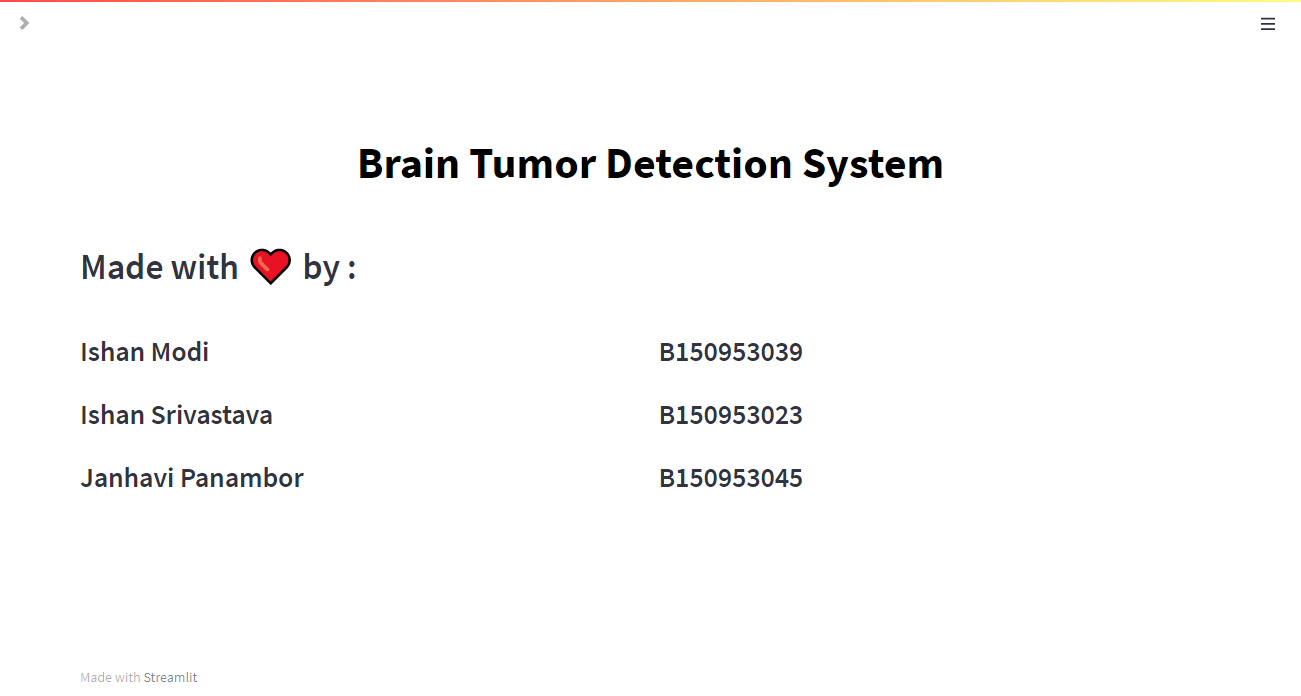
\includegraphics[scale=0.5, angle =90]{Photos/Page5.png}
\caption{Team Information} \label{fig:page5}
\end{figure}

\section{Results from the Web Application}
\begin{itemize}
    \item Glioma Tumour Present in the Brain:
          The figure \ref{fig:glioma_res_web} displays the result on the Web Application when the User uploads a MRI Scan which is of glioma type.
        \begin{figure}[H]
        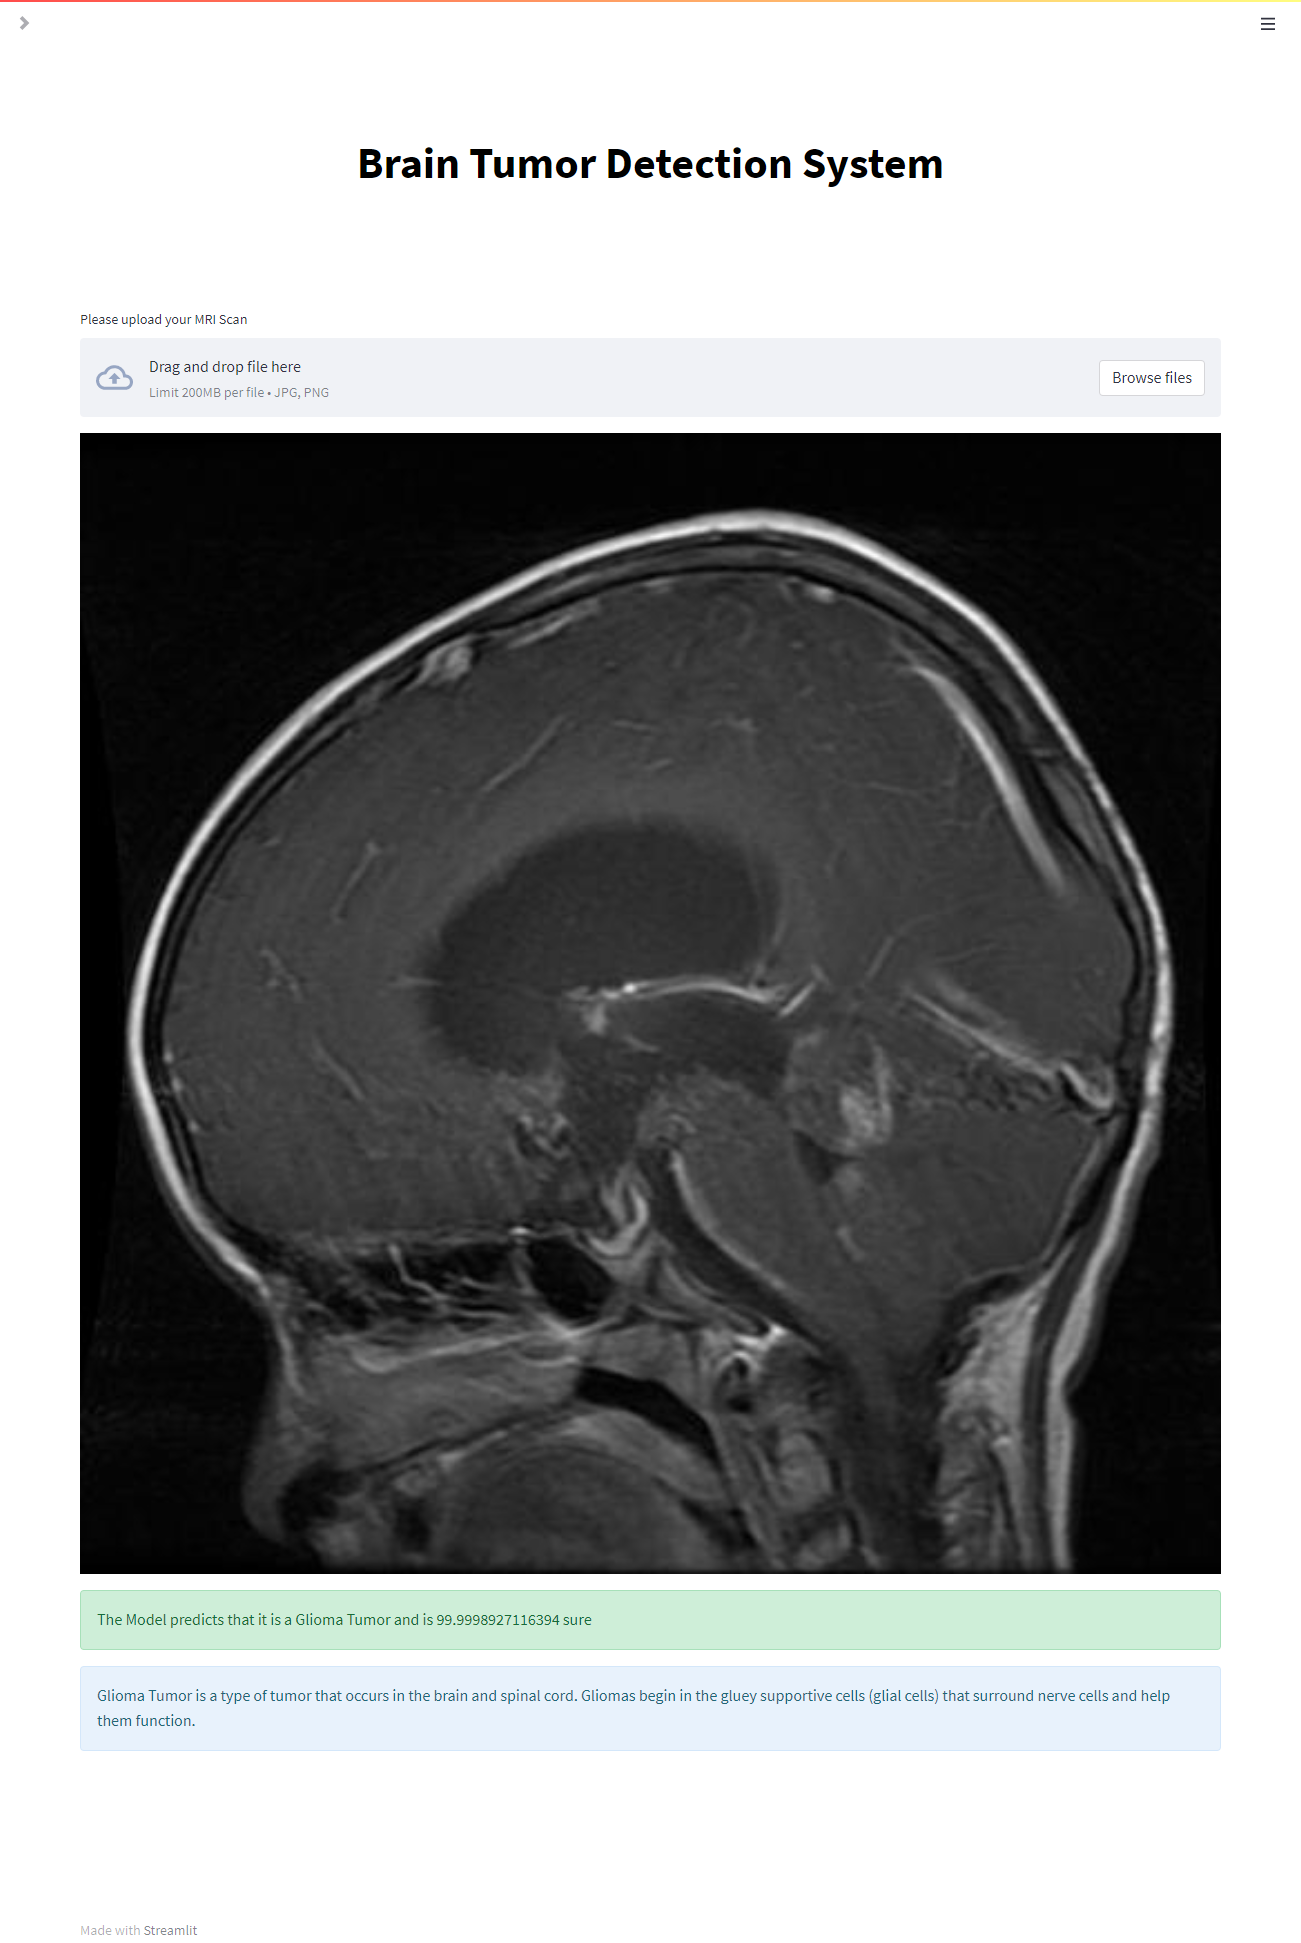
\includegraphics[scale=0.3]{Photos/Resule_glio_web.png}
        \caption{Glioma Tumour Web Application Results} \label{fig:glioma_res_web}
        \end{figure} 
        \vfill
    \item Meningioma Tumour Present in the Brain:
        The figure \ref{fig:menin_res_web} displays the result on the Web Application when the User uploads a MRI Scan which is of meningioma type.
        \begin{figure}[H]
        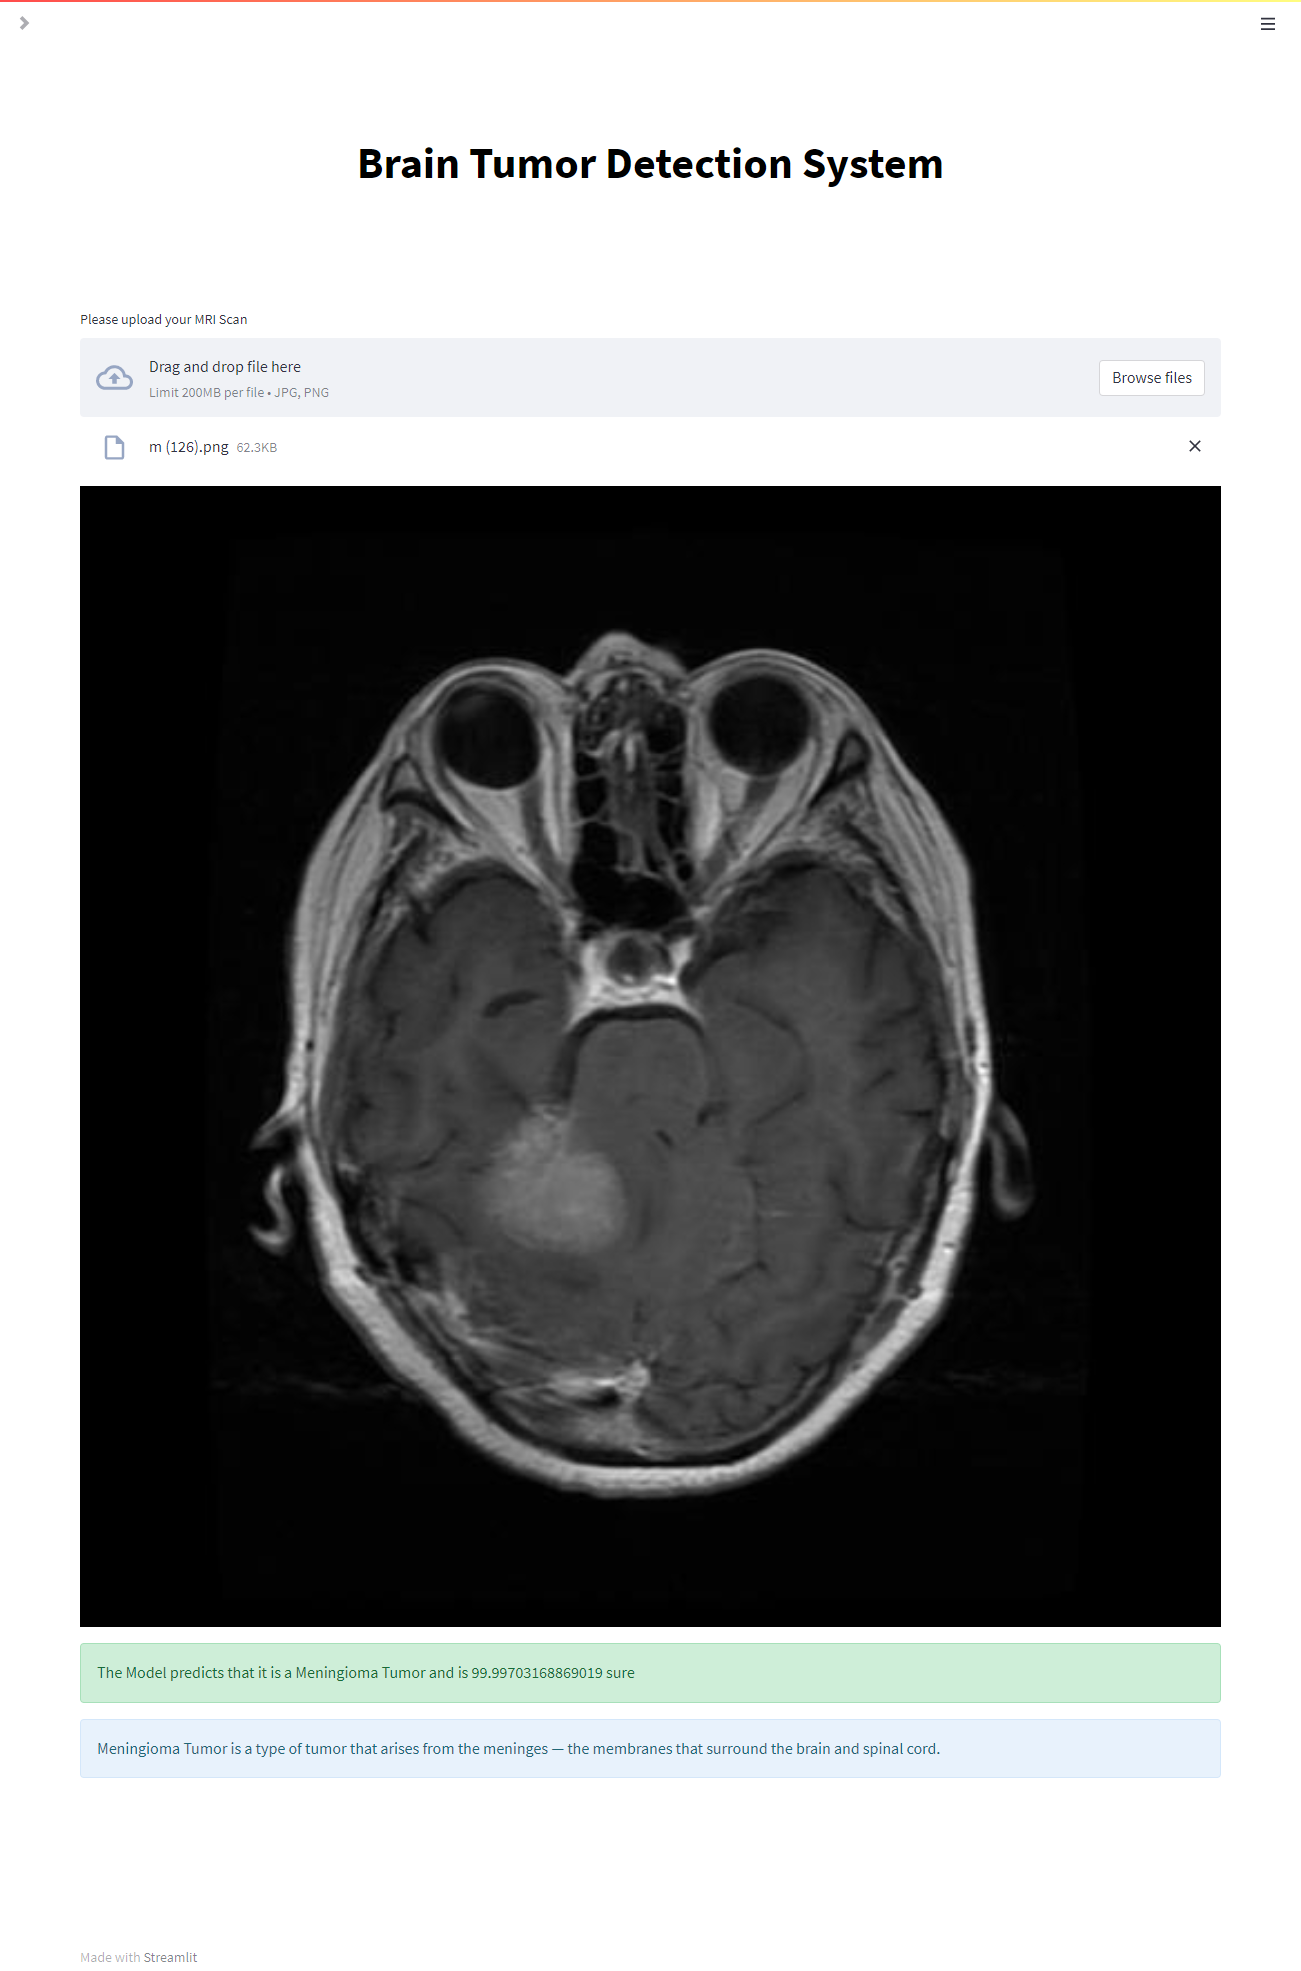
\includegraphics[scale=0.3]{Photos/Resule_meni_web.png}
        \caption{Meningioma Tumour Web Application Results} \label{fig:menin_res_web}
        \end{figure}
        \vfill
    \item Pituitary Tumour Present in the Brain: 
        The figure \ref{fig:pitu_res_web} displays the result on the Web Application when the User uploads a MRI Scan which is of pituitary type.
        \begin{figure}[H]
        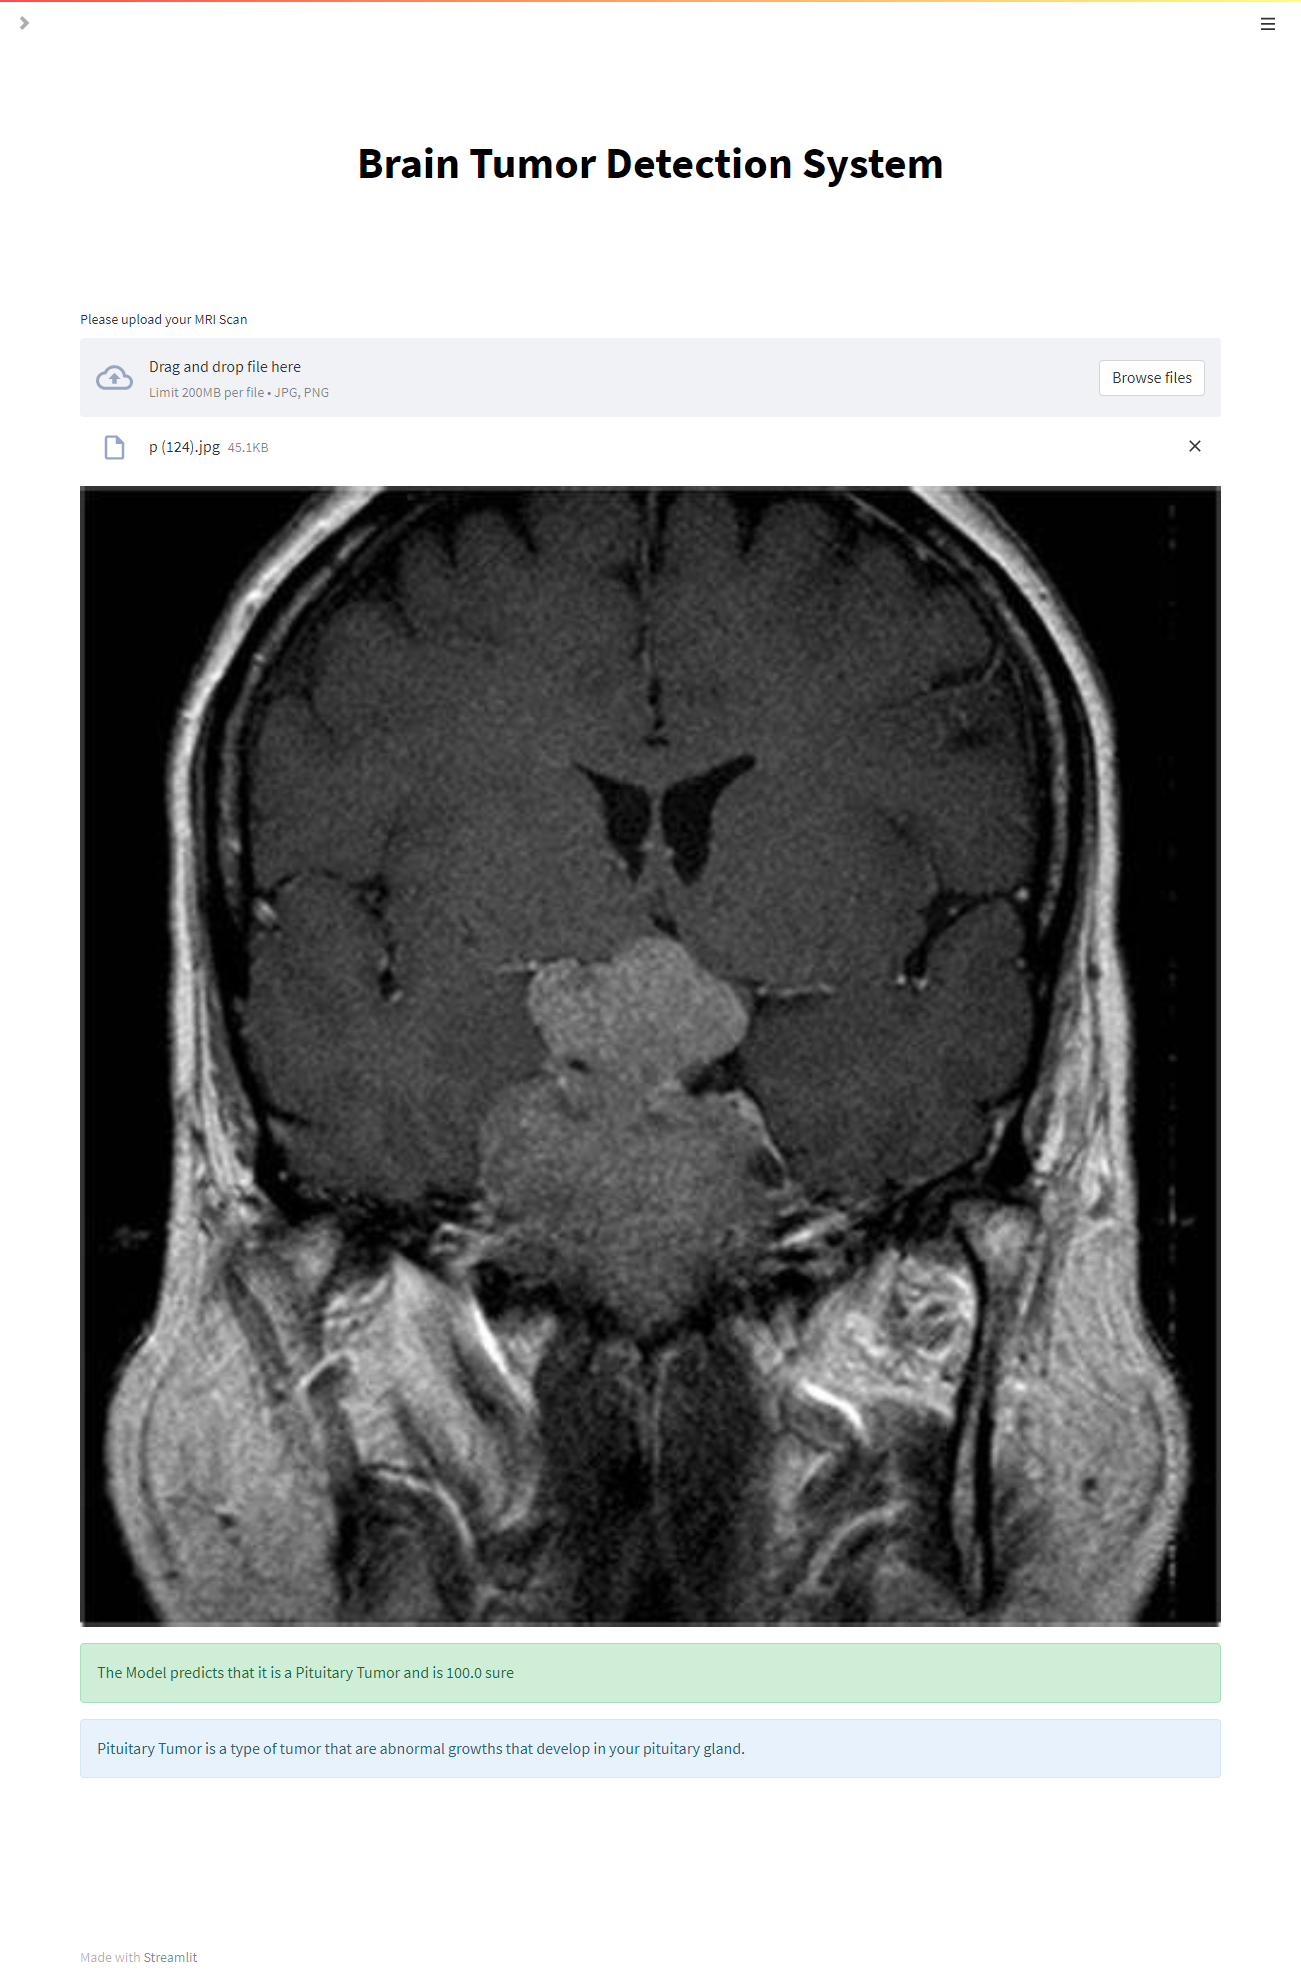
\includegraphics[scale=0.3]{Photos/Resule_pitu_web.png}
        \caption{Pituitary Tumour Web Application Results} \label{fig:pitu_res_web}
        \end{figure}
        \vfill
    \item Tumour Absent in the Brain:
        The figure \ref{fig:no_tumour_res_web} displays the result on the Web Application when the User uploads a MRI Scan which is of non-tumorous type.
        \begin{figure}[H]
        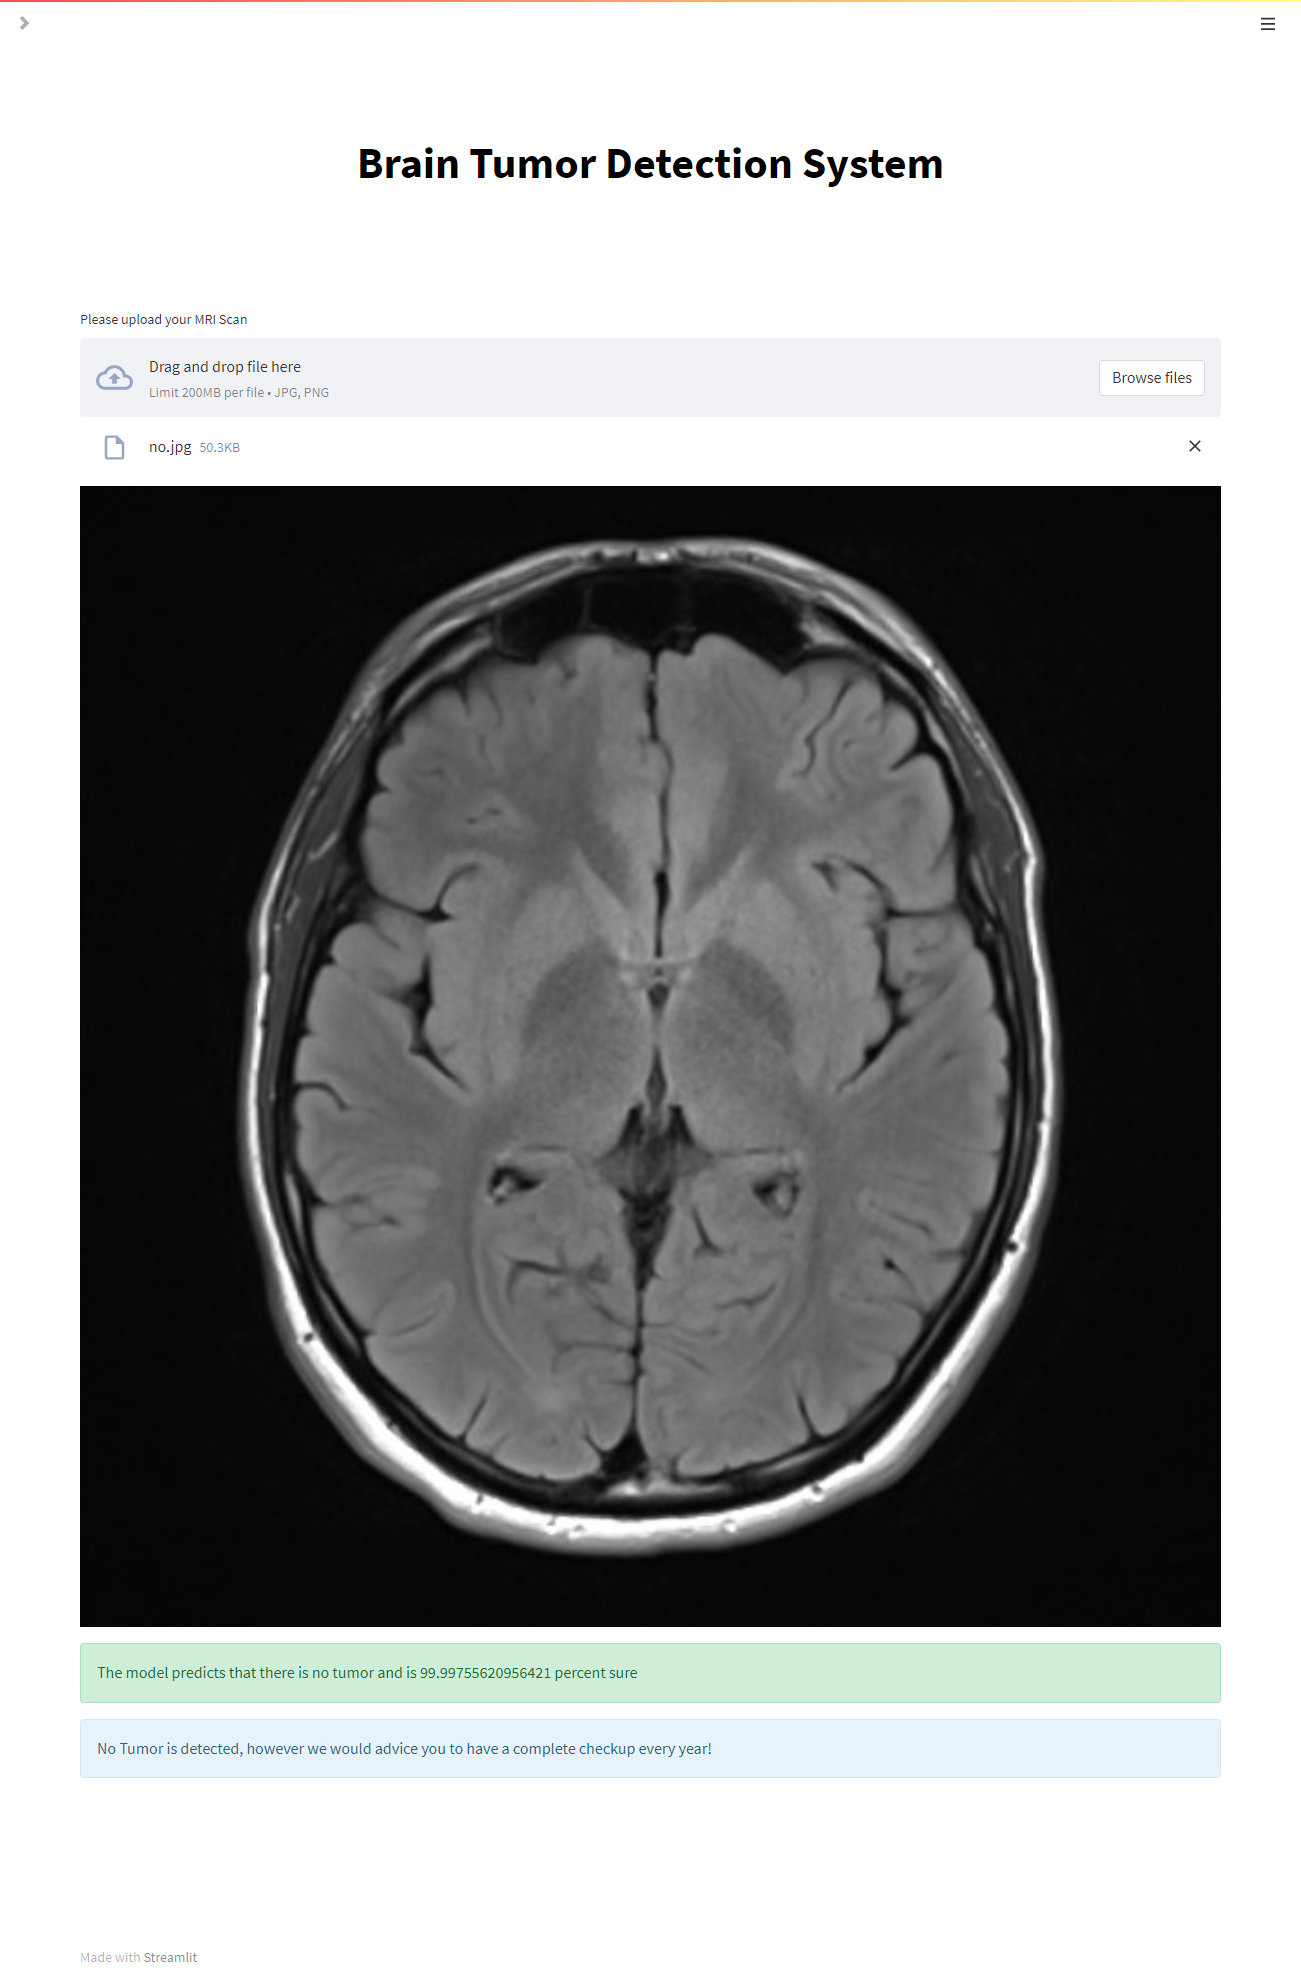
\includegraphics[scale=0.3]{Photos/Resule_no_web.png}
        \caption{No Tumour Web Application Results} \label{fig:no_tumour_res_web}
        \end{figure}   
\end{itemize}


